\documentclass[12pt]{article}

\usepackage{amsmath, color}
\usepackage{mdwmath}
\usepackage{amssymb, epsf, epsfig, textcomp}
\renewcommand{\baselinestretch}{1.3}
\usepackage{a4wide}
\newcommand{\argmin}{\mathop{\mathrm{argmin}}}
\usepackage{caption}
\usepackage{subcaption}
\usepackage{mathtools}
\usepackage{listings}
\lstdefinestyle{myCustomMatlabStyle}{
	basicstyle=\ttfamily\footnotesize,
	breaklines=true,
	language=Matlab,
	numbers=left,
	stepnumber=1,
	numbersep=10pt,
	tabsize=4,
	showspaces=false,
	showstringspaces=false
}
\begin{document}
	\noindent\rule{\textwidth}{2pt}
	\begin{center}
		{\bf Technical University of Crete}\\
		{\bf School of Electrical and Computer Engineering} \\
		Course: {\bf Wireless Communications 2022-2023} \\
		Exercise 1 (100/400) \\
		Report Delivery Date: 10 November 2022 \\
		Instructor: Athanasios P. Liavas \\
	\end{center}
	{\bf Student: }Alevrakis Dimitrios 2017030001\\
	\rule{\textwidth}{.5pt}
	\vskip .1cm
	\noindent
	
	\begin{enumerate}
		\item [\bf 1] We create a flat fading complex channel utilizing the AR-1 model.
		\begin{align*}
			&h[k]=b\cdot h[k-1]+e[k],\ k=1,...,N\\
			&\text{where,}\\
			&h[1]=0\\
			&0<b<1\\
			&R_h[0] \coloneq E[|h[k]|^2]=1\\
			&e[k]\ i.i.d\ \ \mathcal{CN}(0,\sigma_e^2)
		\end{align*}
	
		Calculation of $\sigma_e^2$:
		\begin{align*}
			&E[|h[k]|^2]=R_h[0]\iff\\
			&E[|bh[k-1]|+e[k]|^2]=R_h[0]\iff\\
			&E[|bh[k-1|^2]]+E[|e[k]|^2]\ge R_h[0]\iff\\
			&b^2R_h[0]+\sigma_e^2\ge R_h[0]\iff\\
			&\sigma_e^2\ge R_h[0](1-b^2)
		\end{align*}
		Therefore we can choose $\sigma_e^2=R_h[0](1-b^2)$
		
		\begin{figure}
			\centering
			\begin{subfigure}[b]{0.8\textwidth}
				\centering
				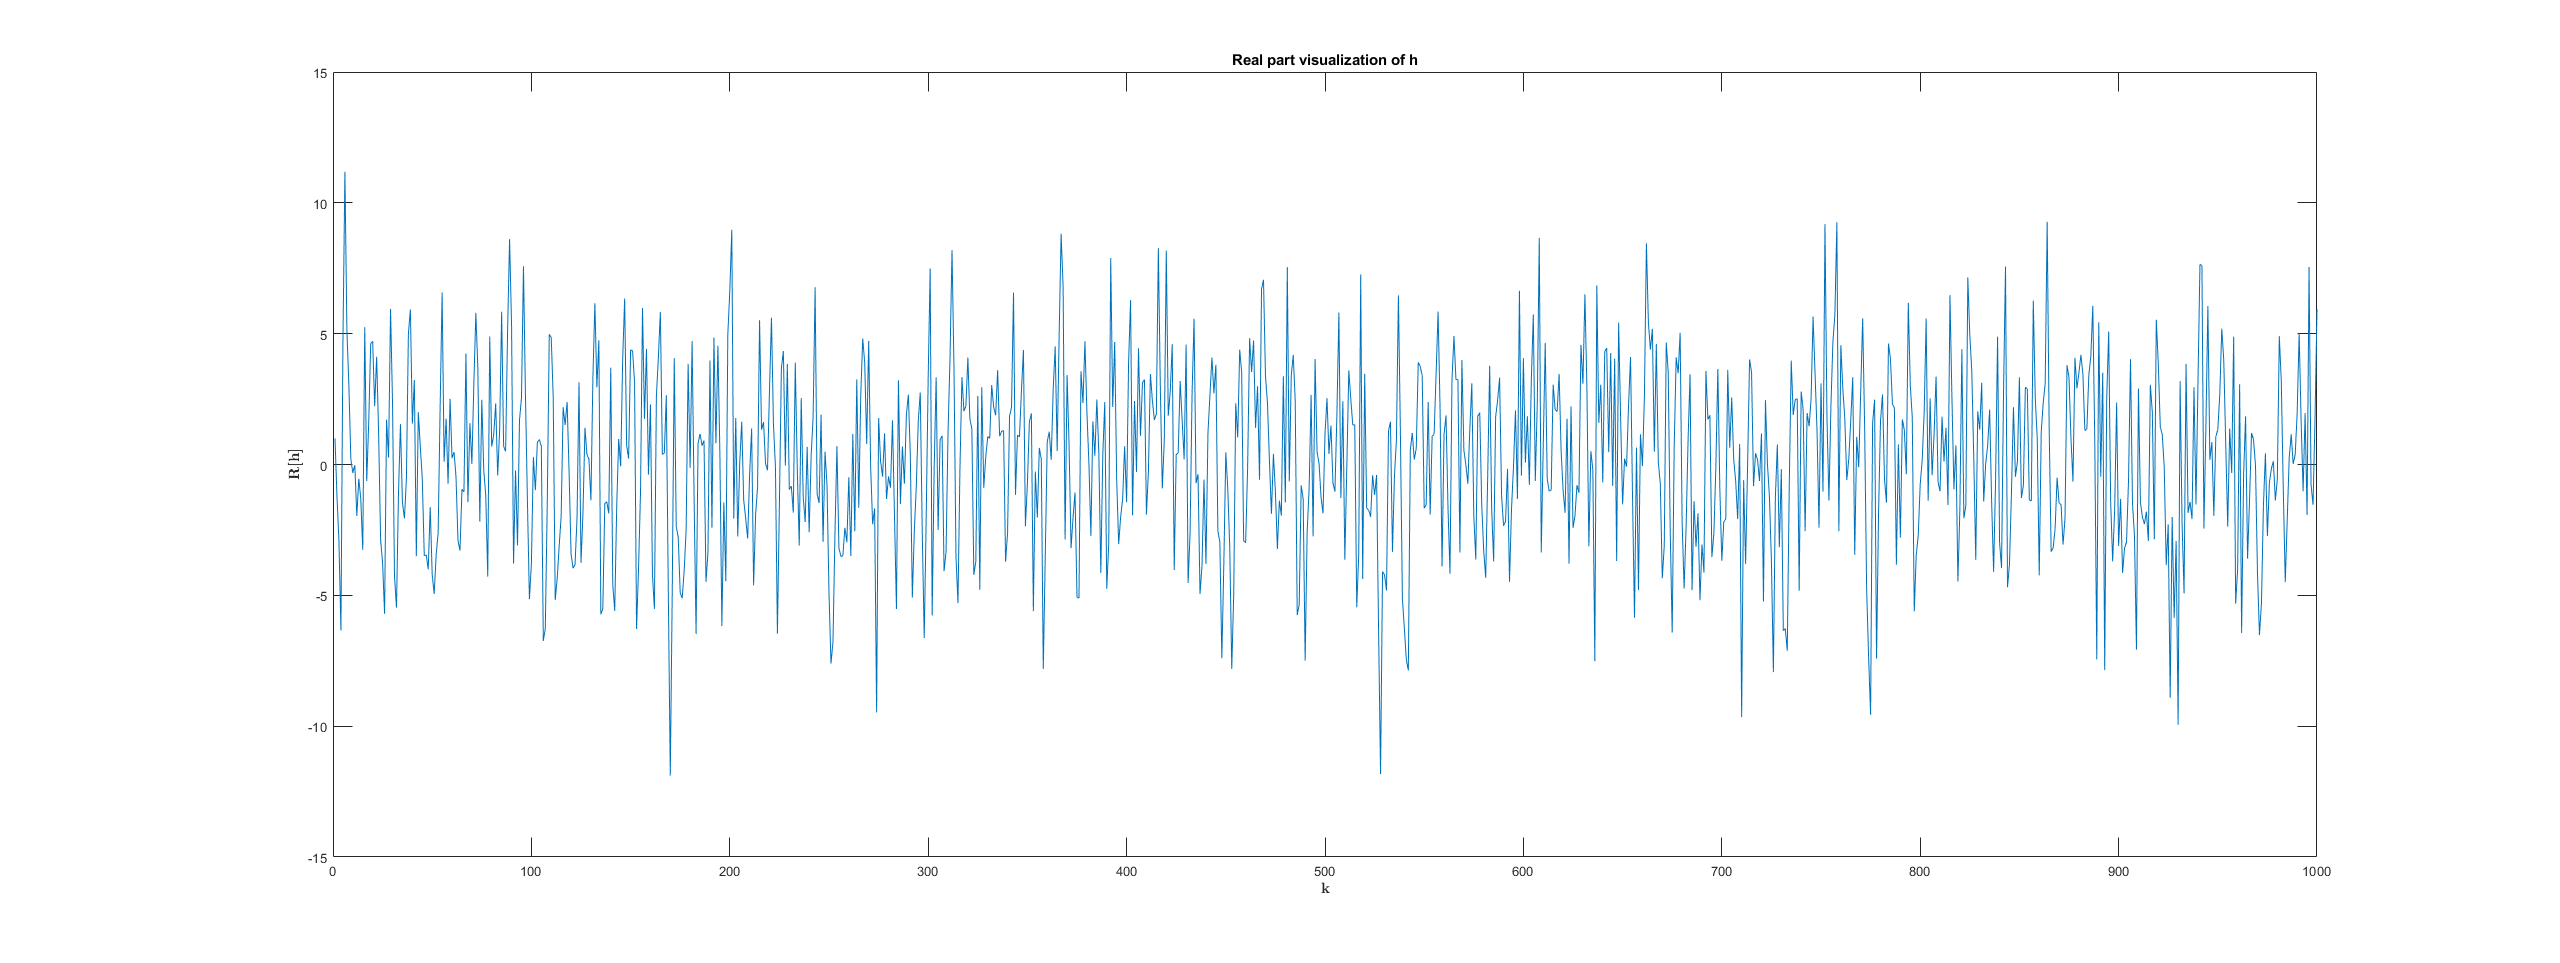
\includegraphics[width=0.9\textwidth]{fig1.png}
			\end{subfigure}
			\begin{subfigure}[b]{0.8\textwidth}
				\centering
				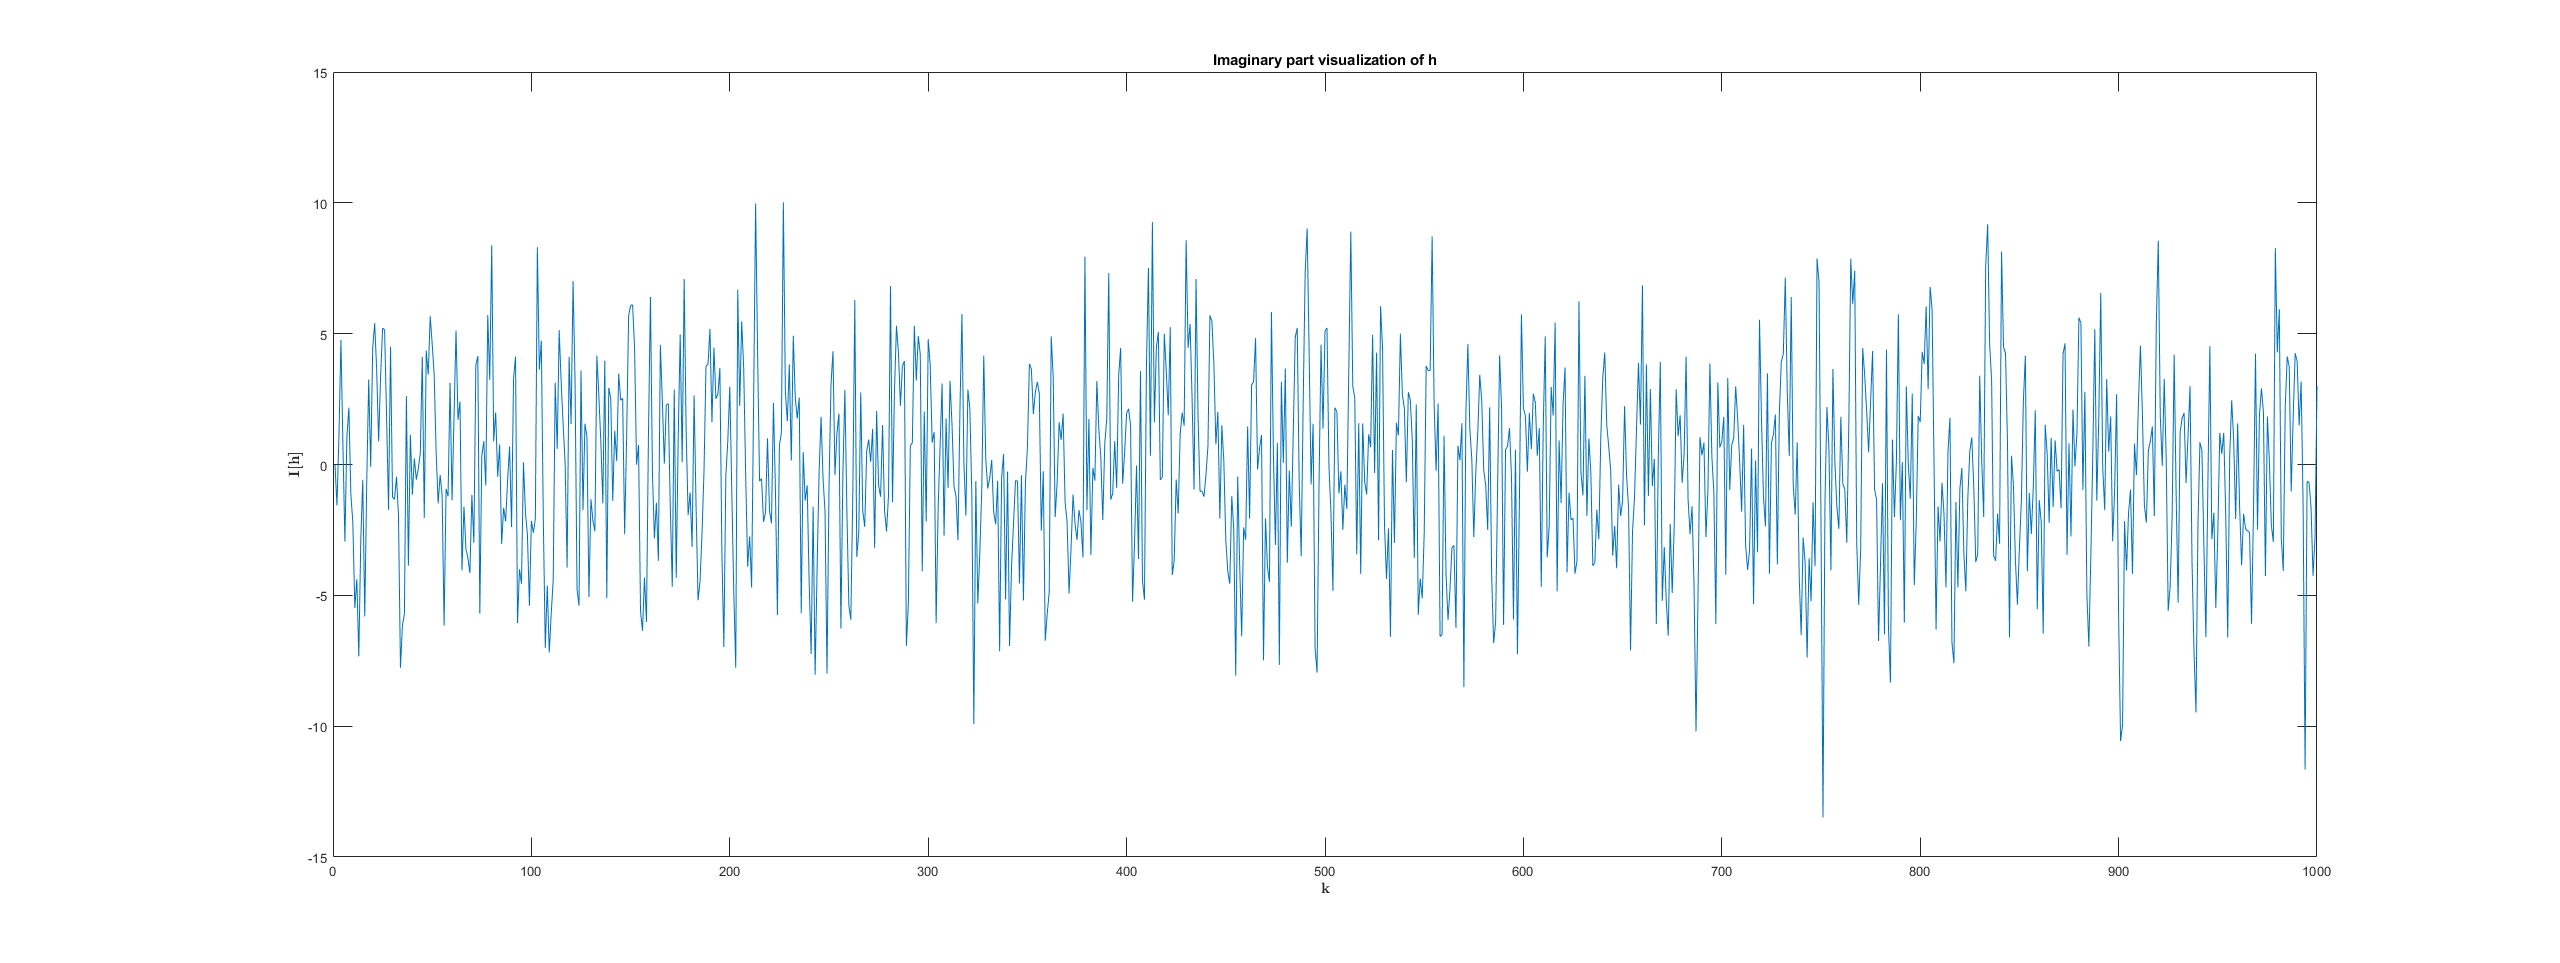
\includegraphics[width=0.9\textwidth]{fig2.png}
			\end{subfigure}
			\caption{$b\ll1$}
		\end{figure}
	
		\begin{figure}
			\centering
			\begin{subfigure}[b]{0.8\textwidth}
				\centering
				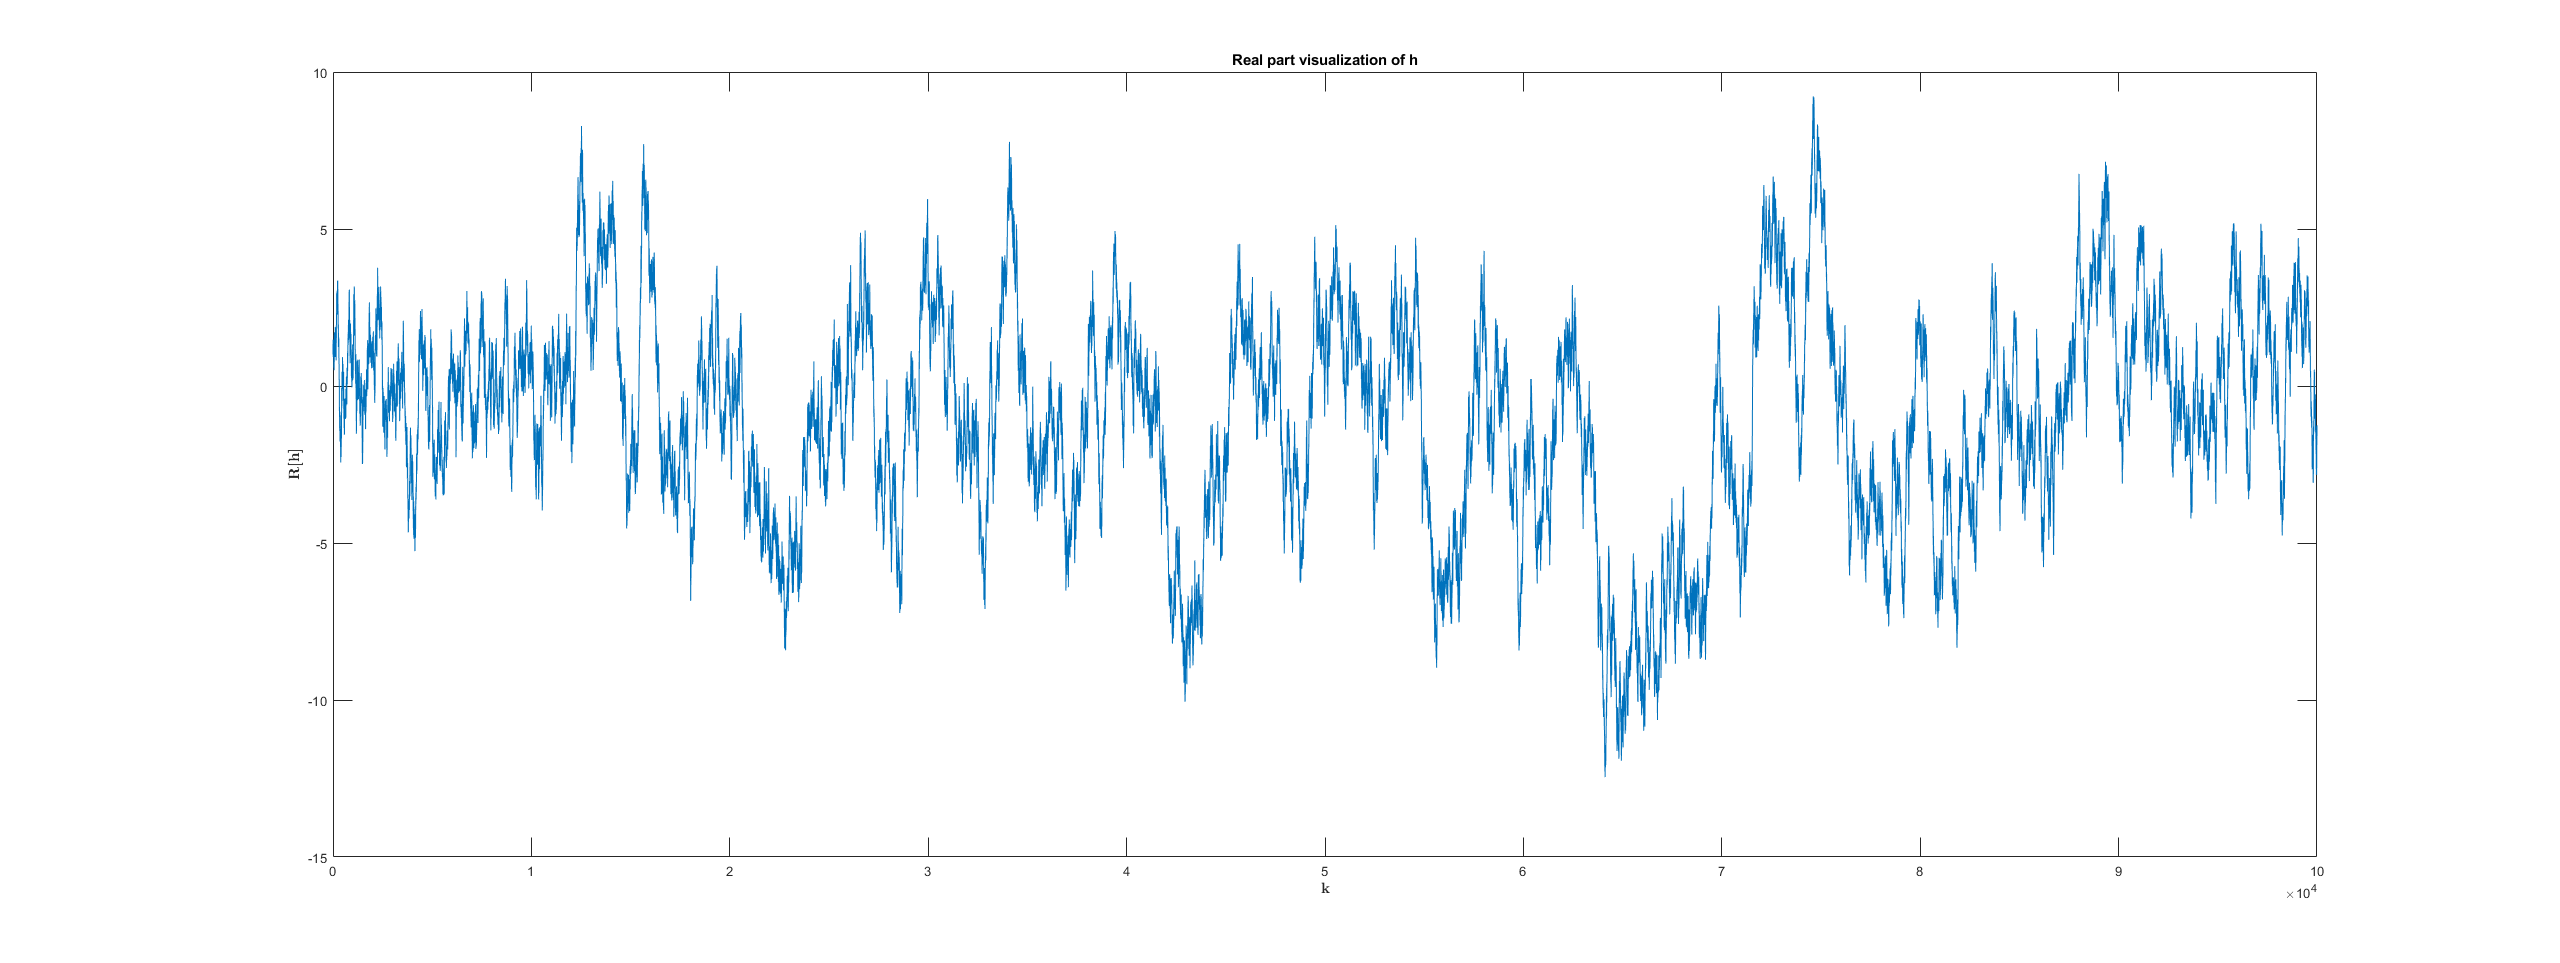
\includegraphics[width=0.9\textwidth]{fig1_b.png}
			\end{subfigure}
			\begin{subfigure}[b]{0.8\textwidth}
				\centering
				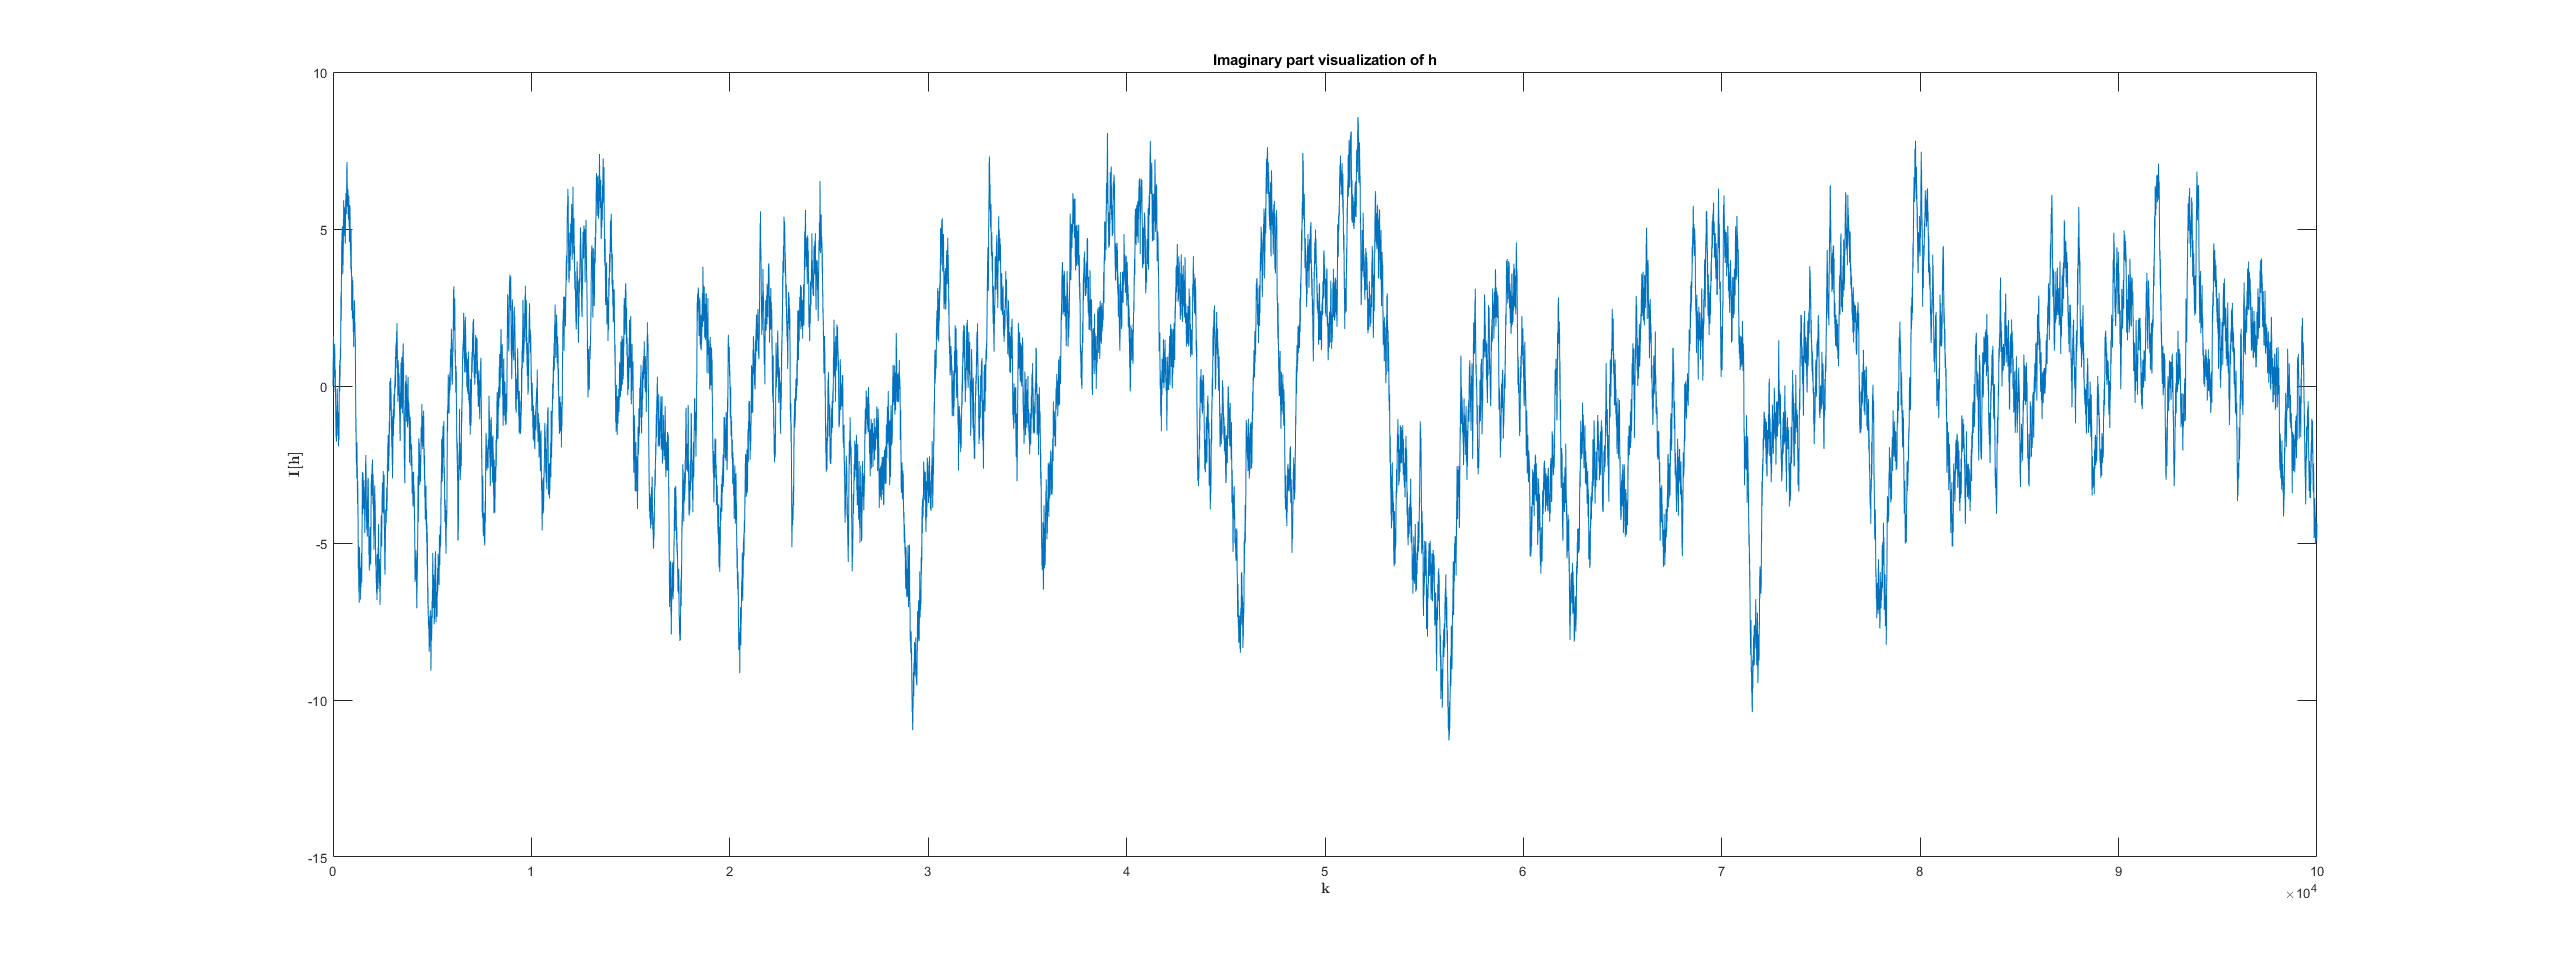
\includegraphics[width=0.9\textwidth]{fig2_b.png}
			\end{subfigure}
			\caption{$b\approx1$}
		\end{figure}
	
		In figures 1 and 2 is evident that for $b\approx1$ the channel takes longer to become stationary and therefore if a mean is taken in a small interval it will be inaccurate. For $b\ll1$ the mean is observable even in smaller intervals even in the first samples.
		\newpage
		\item[\bf 3]
		Calculating the mean received snr:
		\begin{align*}
			SNR=\frac{E[|h[k]s[k]|^2]}{E[|n[k]^2|]}=\frac{E[|h[k]|^2]E[|s[k]|^2]}{E[|n[k]^2|]}=E[|s[k]|^2]=R_h[0]E[|s[k]|^2] = 2R_h[0]
		\end{align*}
		Therefore $SNR_{db} = 10log_{10}2R_h[0]$
		
		\item[\bf 4]
		Using the Maximum Likelihood (ML) method we arrive at the following rule:
		\begin{align*}
			\underset{x\in4-QAM}{max}f_{Y|X=x}(y)=\underset{x\in4-QAM}{min}|y-hx|^2
		\end{align*}
		Therefore we choose the $x\in4-QAM$ closest to $r[k]$
		\newpage
		\item[\bf 5]
		\begin{figure}
			\centering
			\begin{subfigure}[b]{\textwidth}
				\centering
				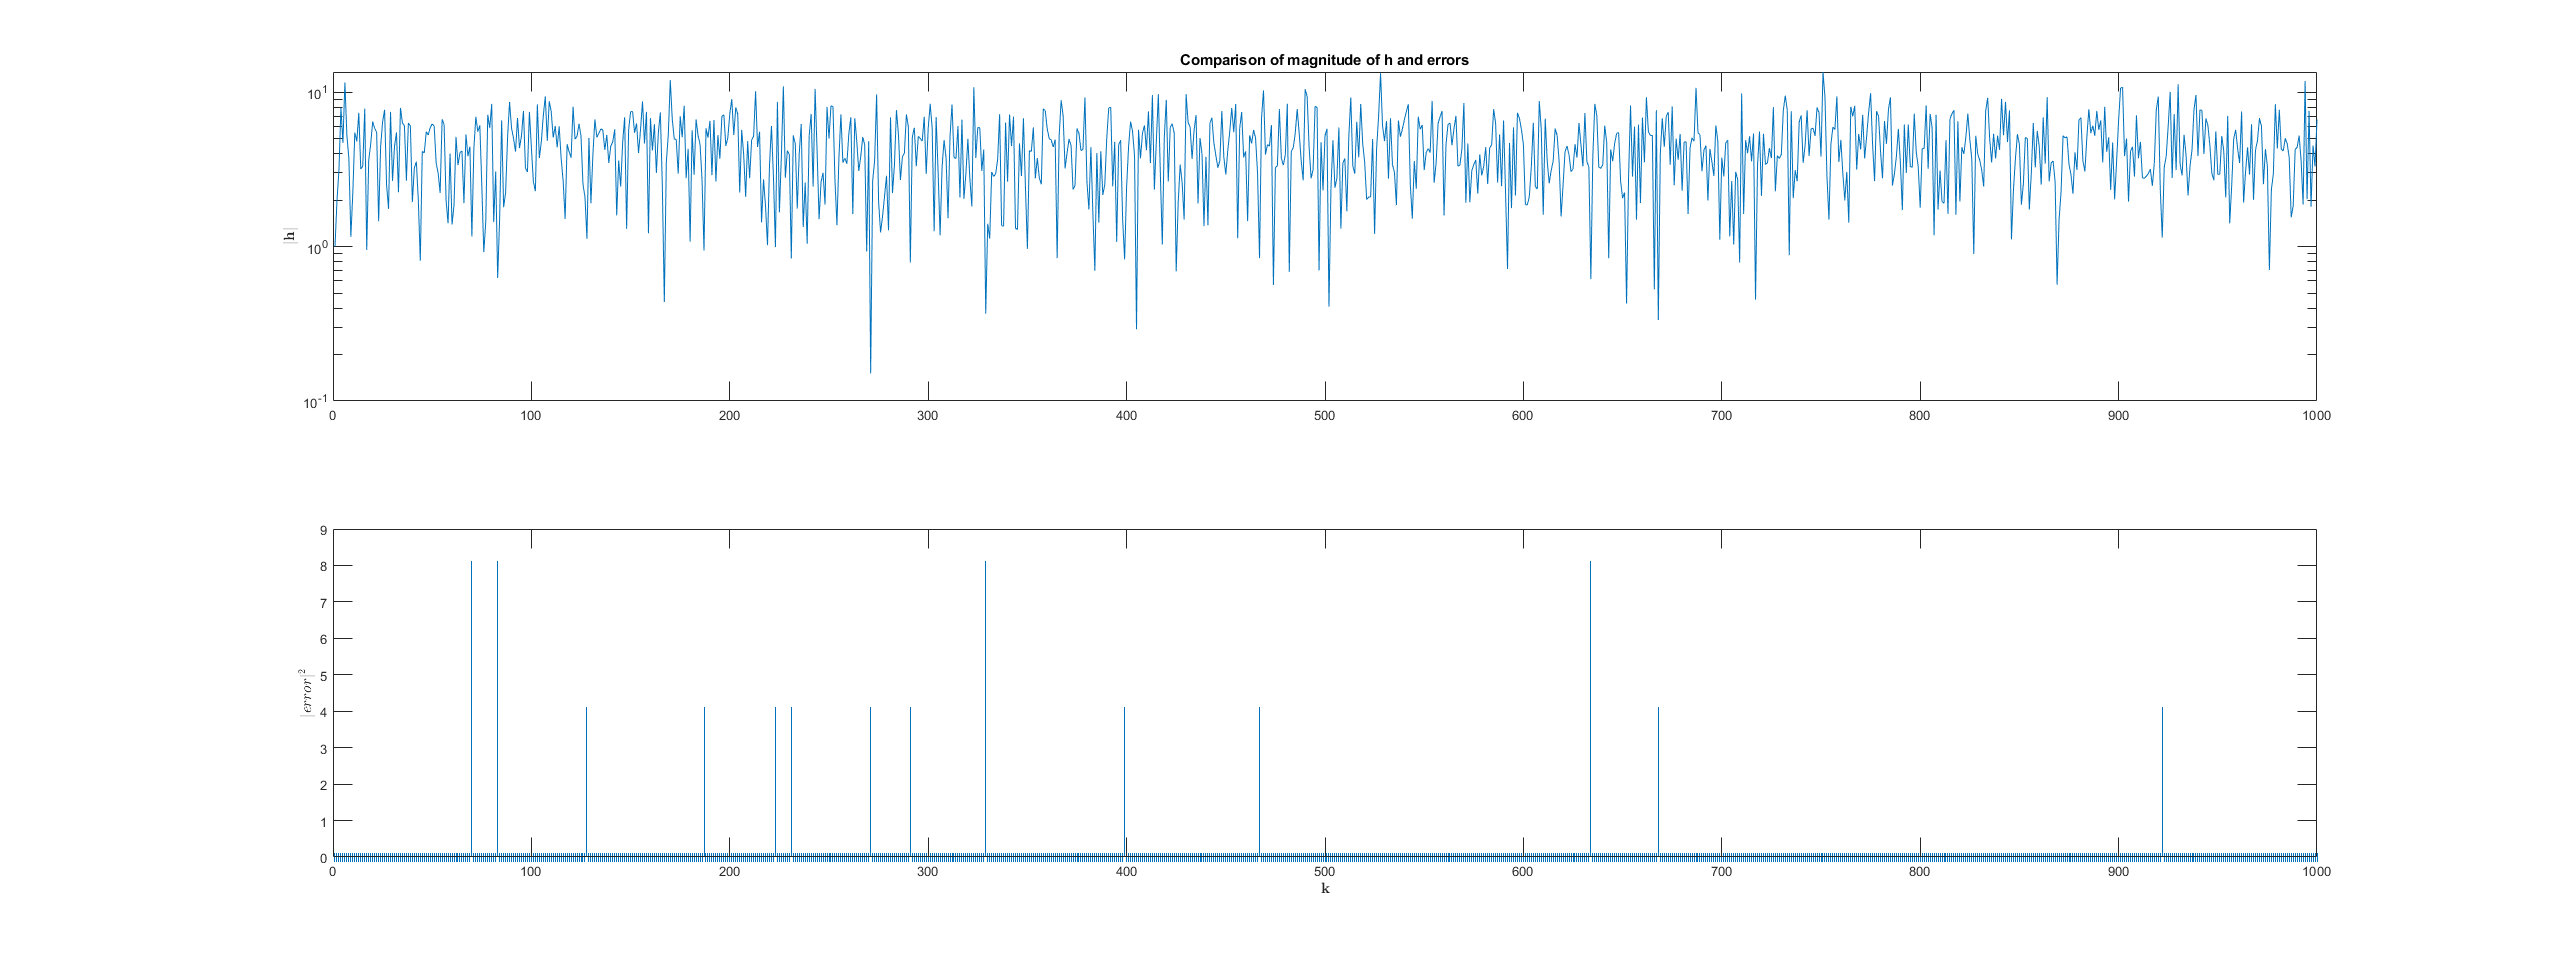
\includegraphics[width=0.9\textwidth]{fig3.png}
				\caption{$b\ll1$}
			\end{subfigure}
			\begin{subfigure}[b]{\textwidth}
				\centering
				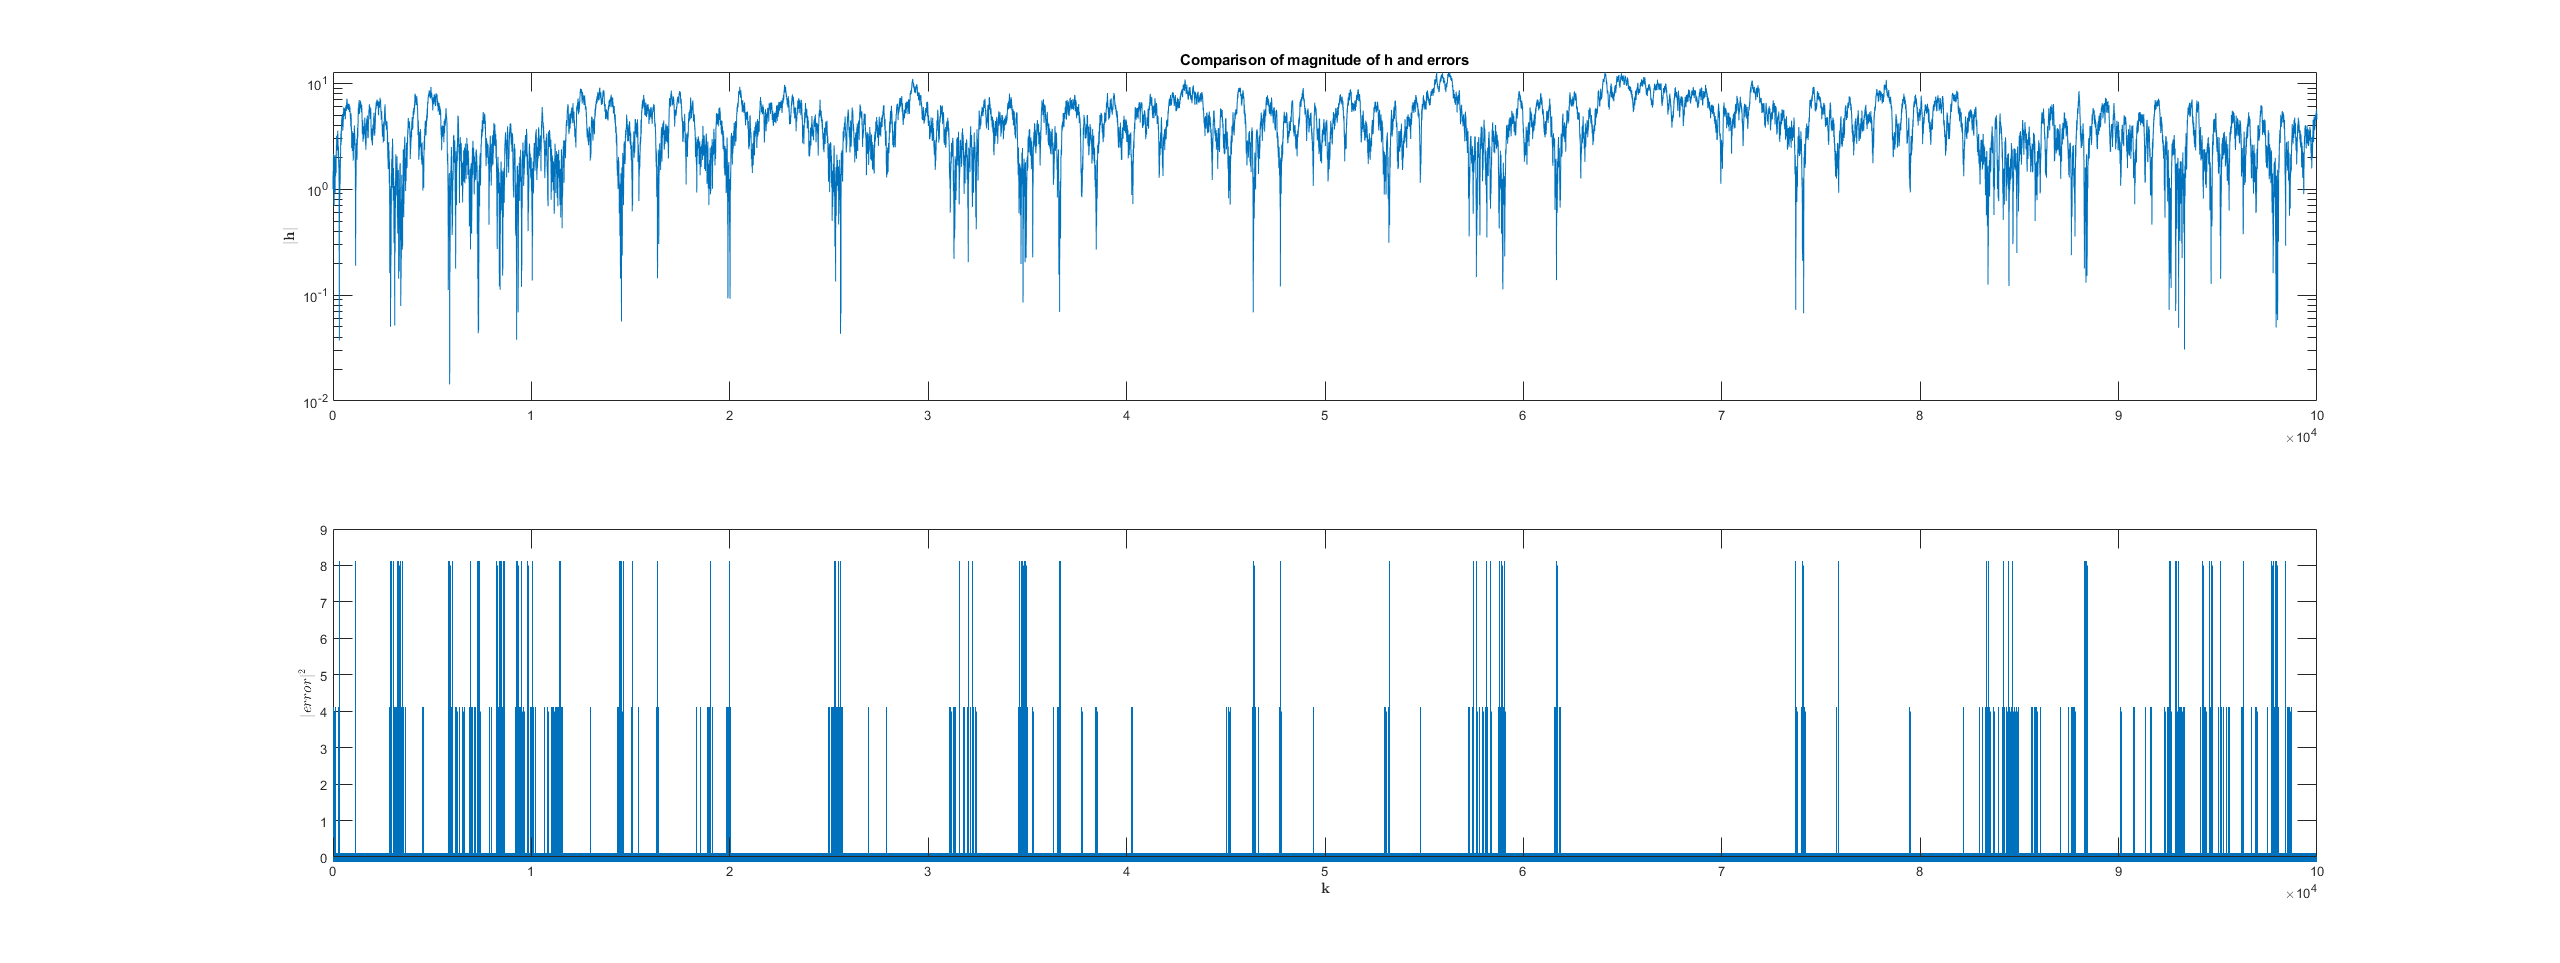
\includegraphics[width=0.9\textwidth]{fig3_b.png}
				\caption{$b\approx1$}
			\end{subfigure}
			\caption{$SNR_{db}\approx17$}
		\end{figure}
		We observe that for both cases of $b$ and for $SNR_{db}>15$ that the errors are grouped around the points that the channel has the lowest magnitudes.
		
		\newpage
		\item[\bf 6]
		From (figure 3) the channel seems to create more "prominent" lows regarding its magnitudes for $b\approx1$, (because in this case the channel "takes" longer to become stationary). Therefore the errors are more grouped together.
	
		\item[\bf 7]
		\begin{figure}[h!]
		\centering
		\begin{subfigure}[b]{\textwidth}
			\centering
			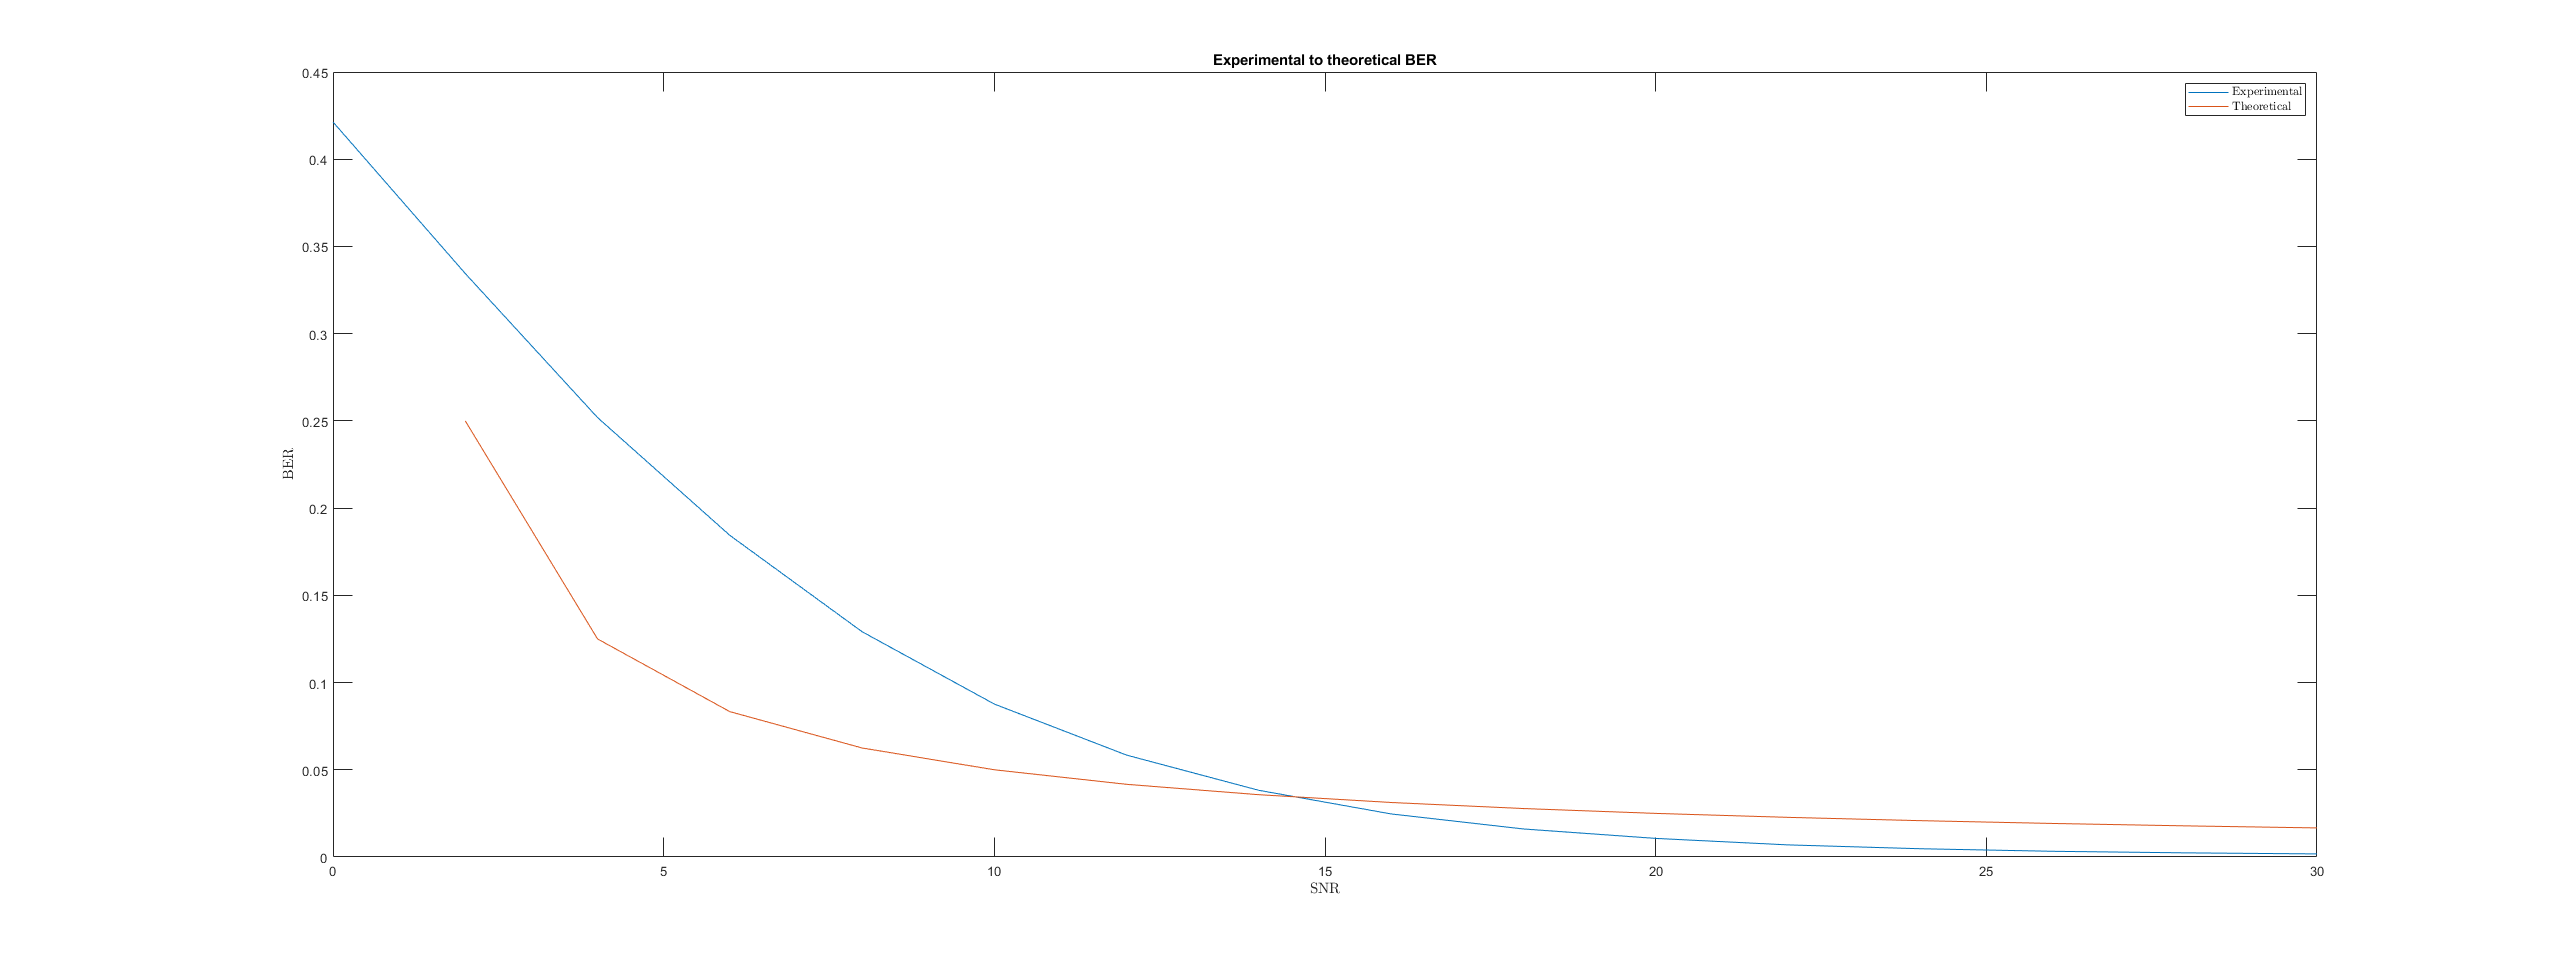
\includegraphics[width=0.9\textwidth]{fig4.png}
		\end{subfigure}
		\begin{subfigure}[b]{\textwidth}
			\centering
			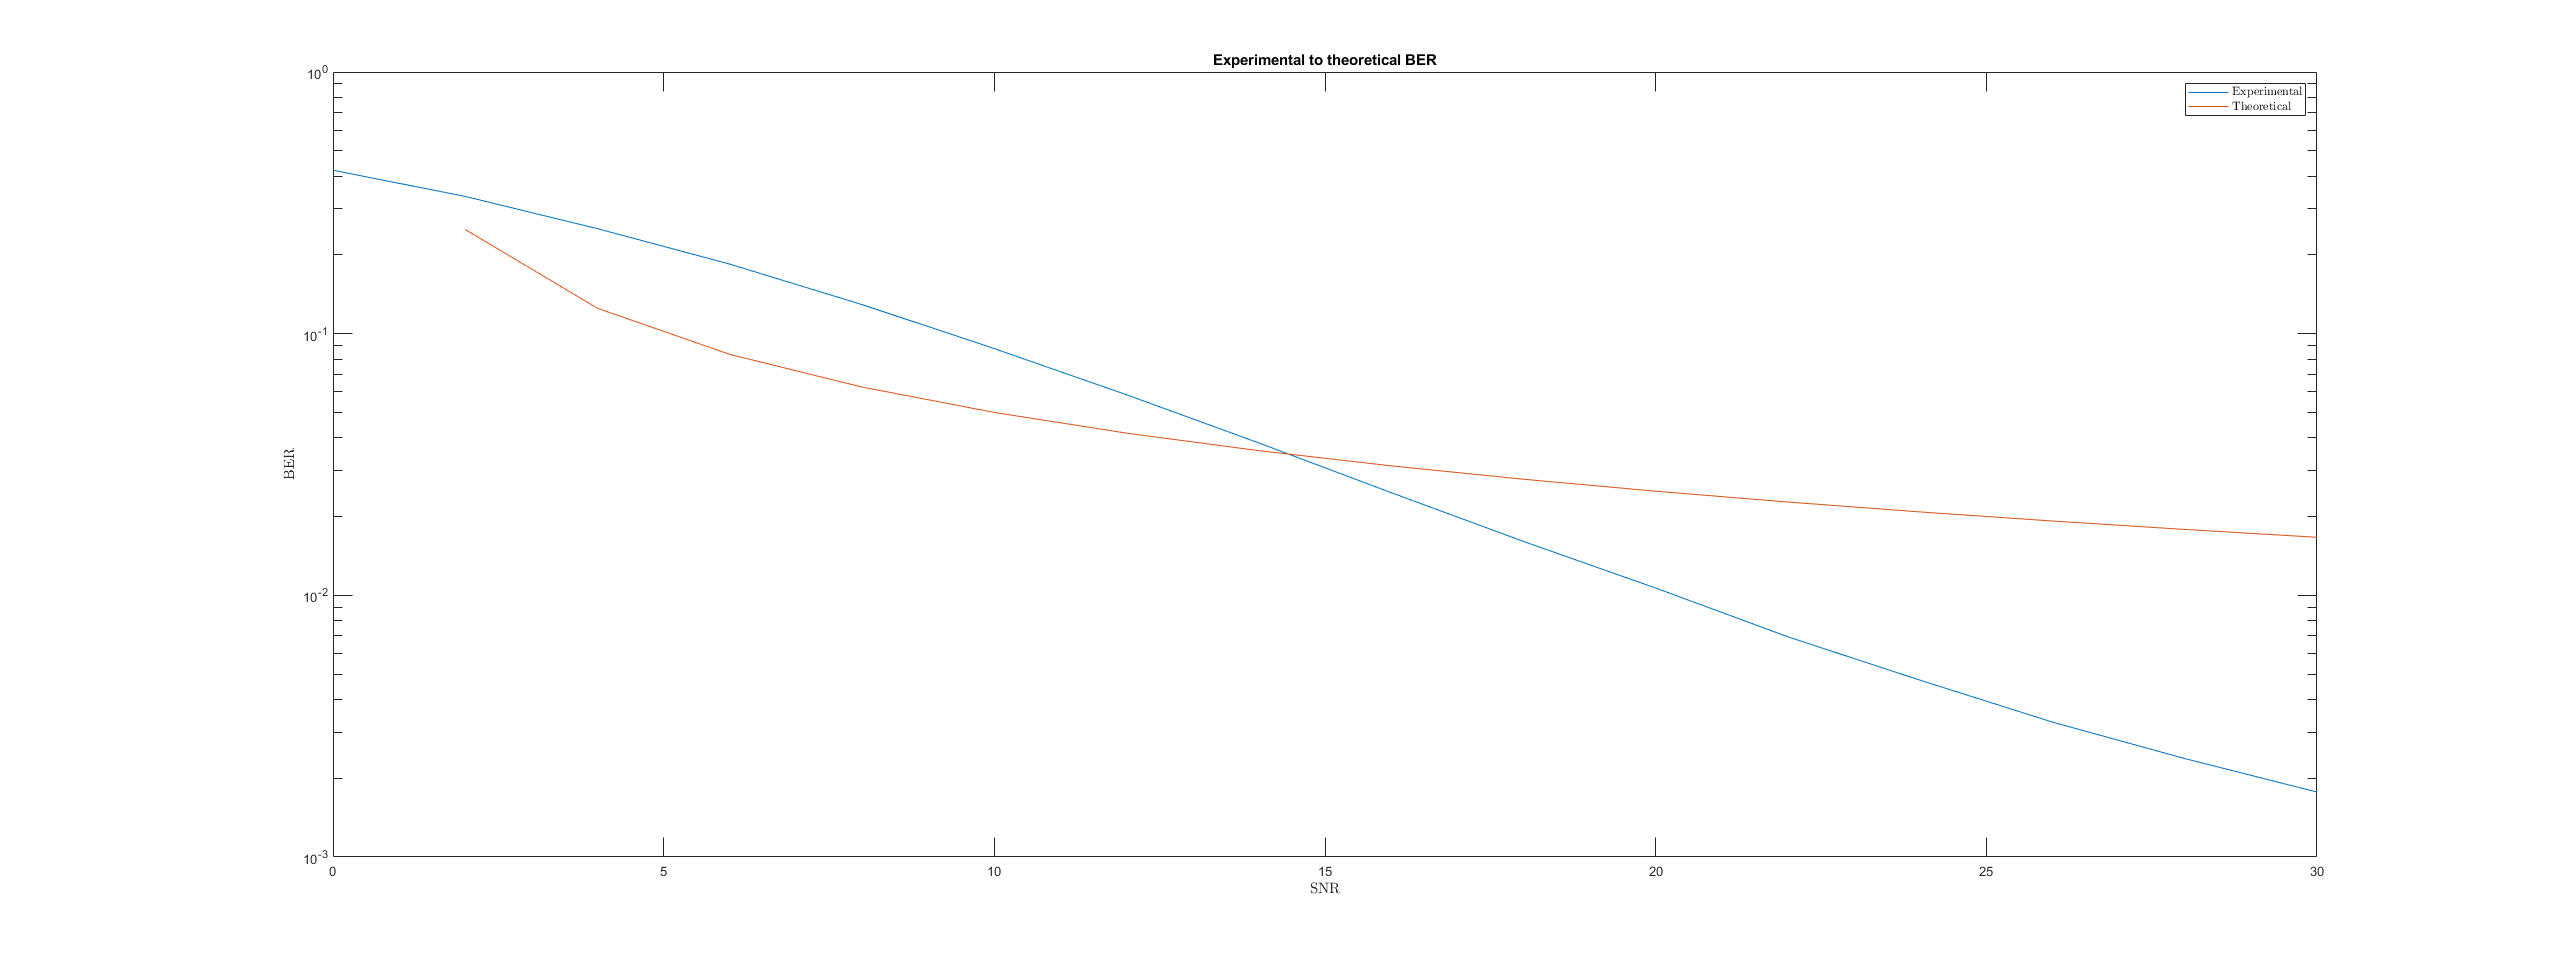
\includegraphics[width=0.9\textwidth]{fig4_b.png}
		\end{subfigure}
		\caption{$b\ll 1$}
		\end{figure}
		By observing the regular and semi-log scale plots in (figure 4) we can see that the BER decreases significantly when increasing the SNR.
		
		\newpage
		\item[\bf 8]
		\begin{figure}
			\centering
			\begin{subfigure}[b]{\textwidth}
				\centering
				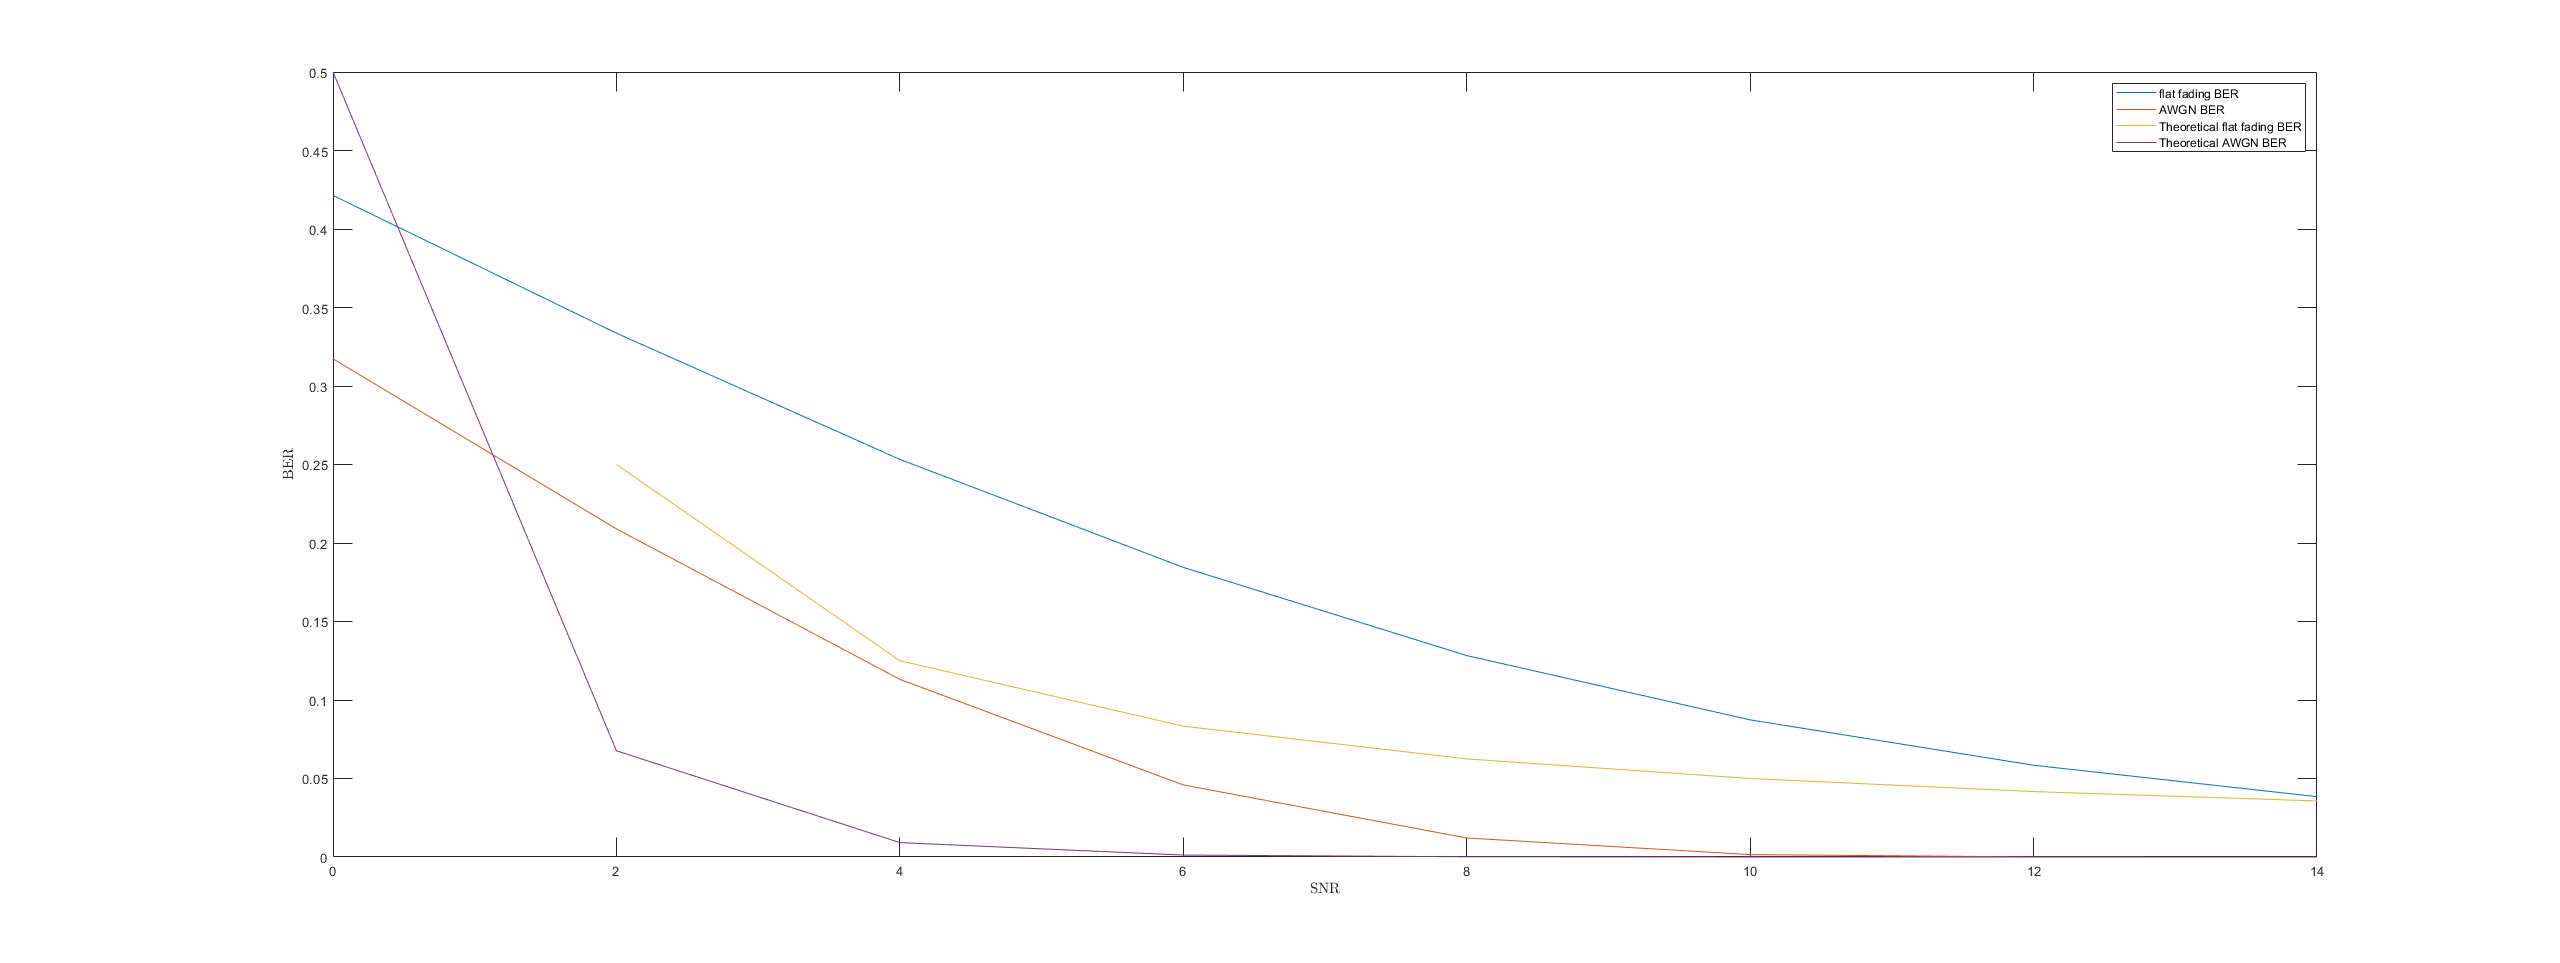
\includegraphics[width=0.9\textwidth]{fig5.png}
			\end{subfigure}
			\begin{subfigure}[b]{\textwidth}
				\centering
				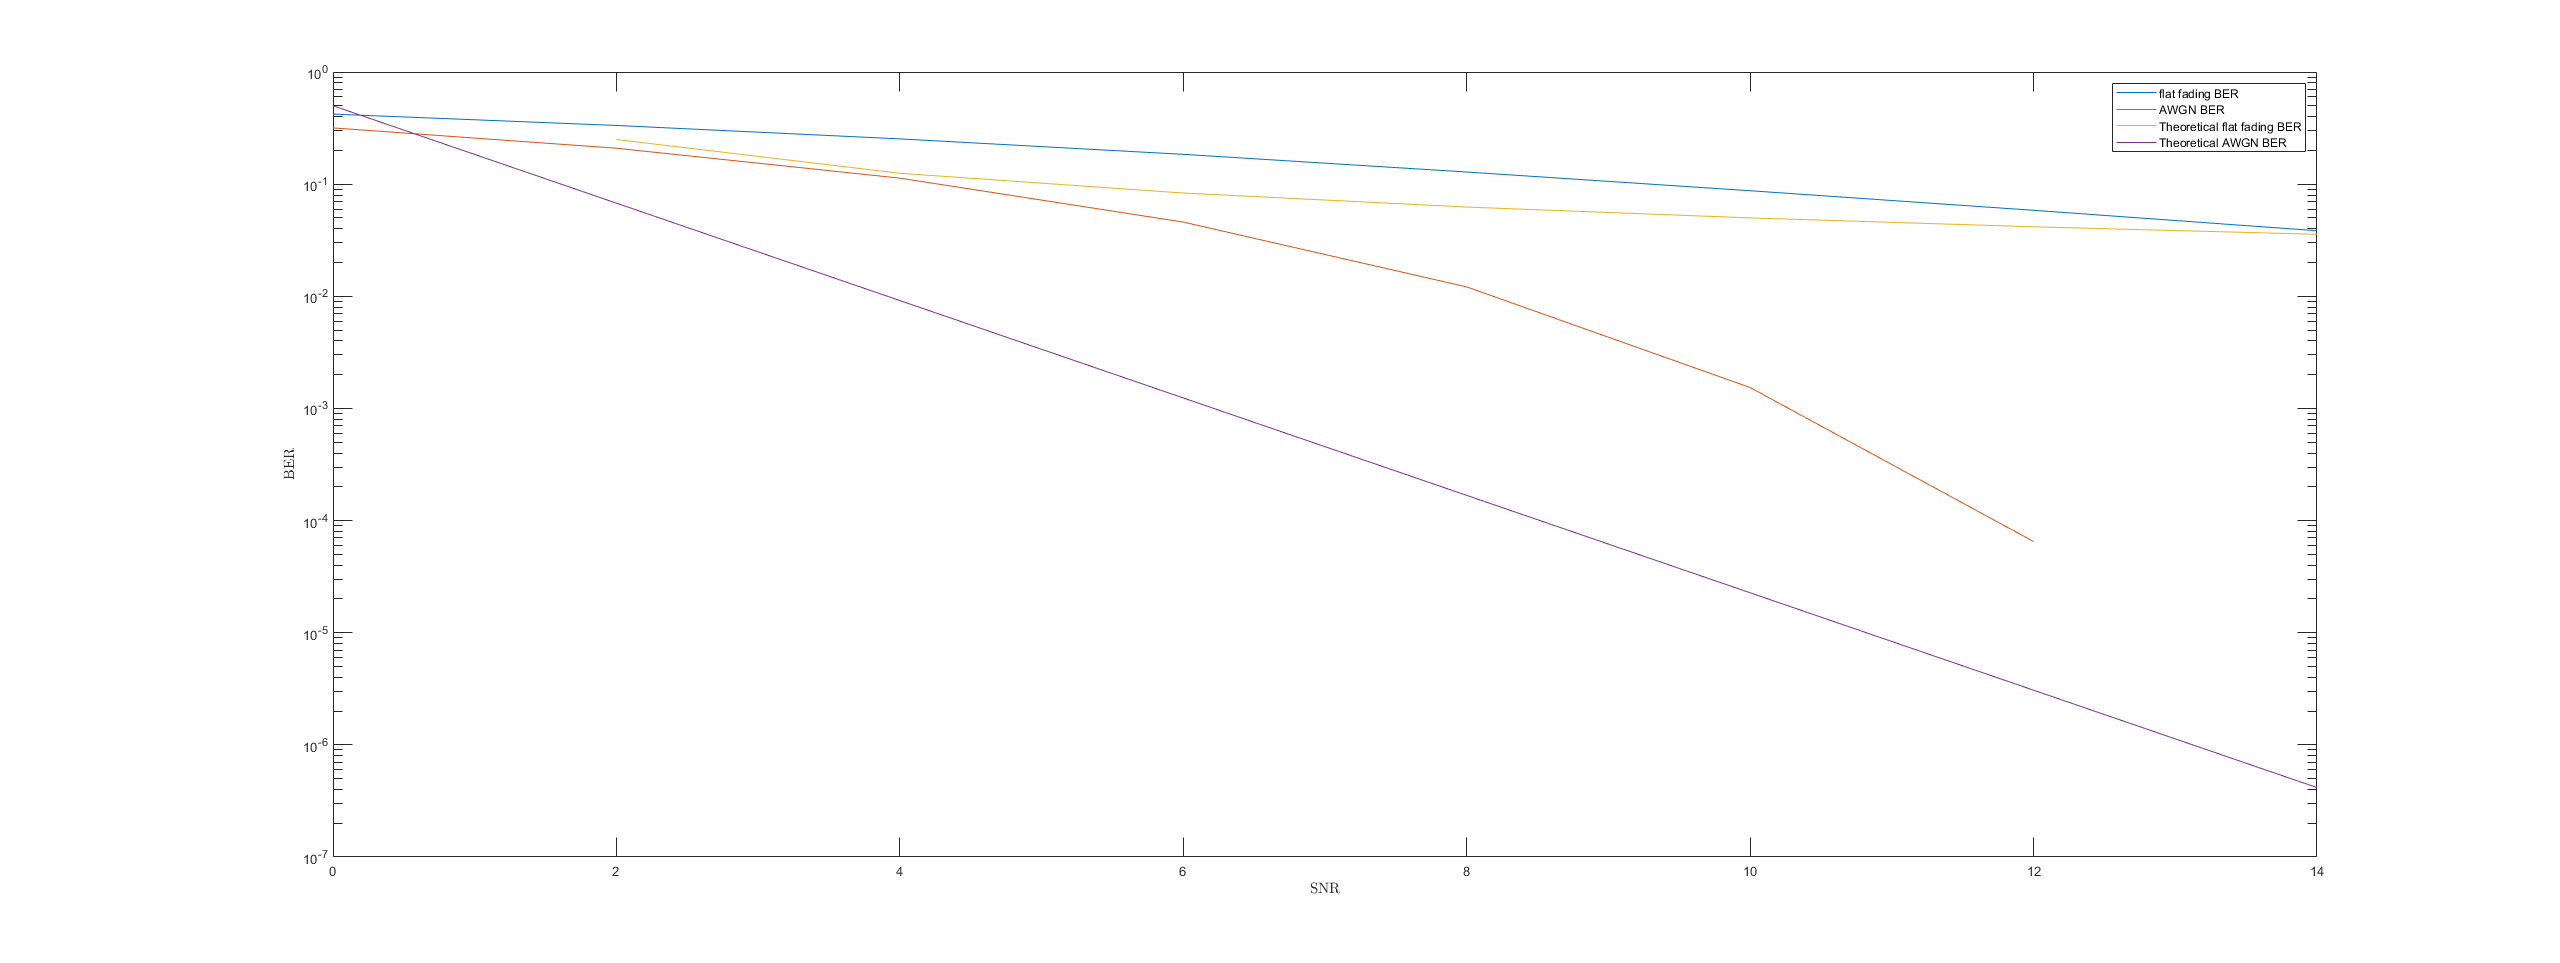
\includegraphics[width=0.9\textwidth]{fig5_b.png}
			\end{subfigure}
			\caption{$b\ll 1$}
		\end{figure}
		Again in every case BER decreases for higher SNRs and,\\
		as expected the AWGN model performs better than the flat fading since it does not account for the fading. 
		
		\newpage
		\begin{figure}[h!]
			\centering
			\begin{subfigure}[b]{0.8\textwidth}
				\centering
				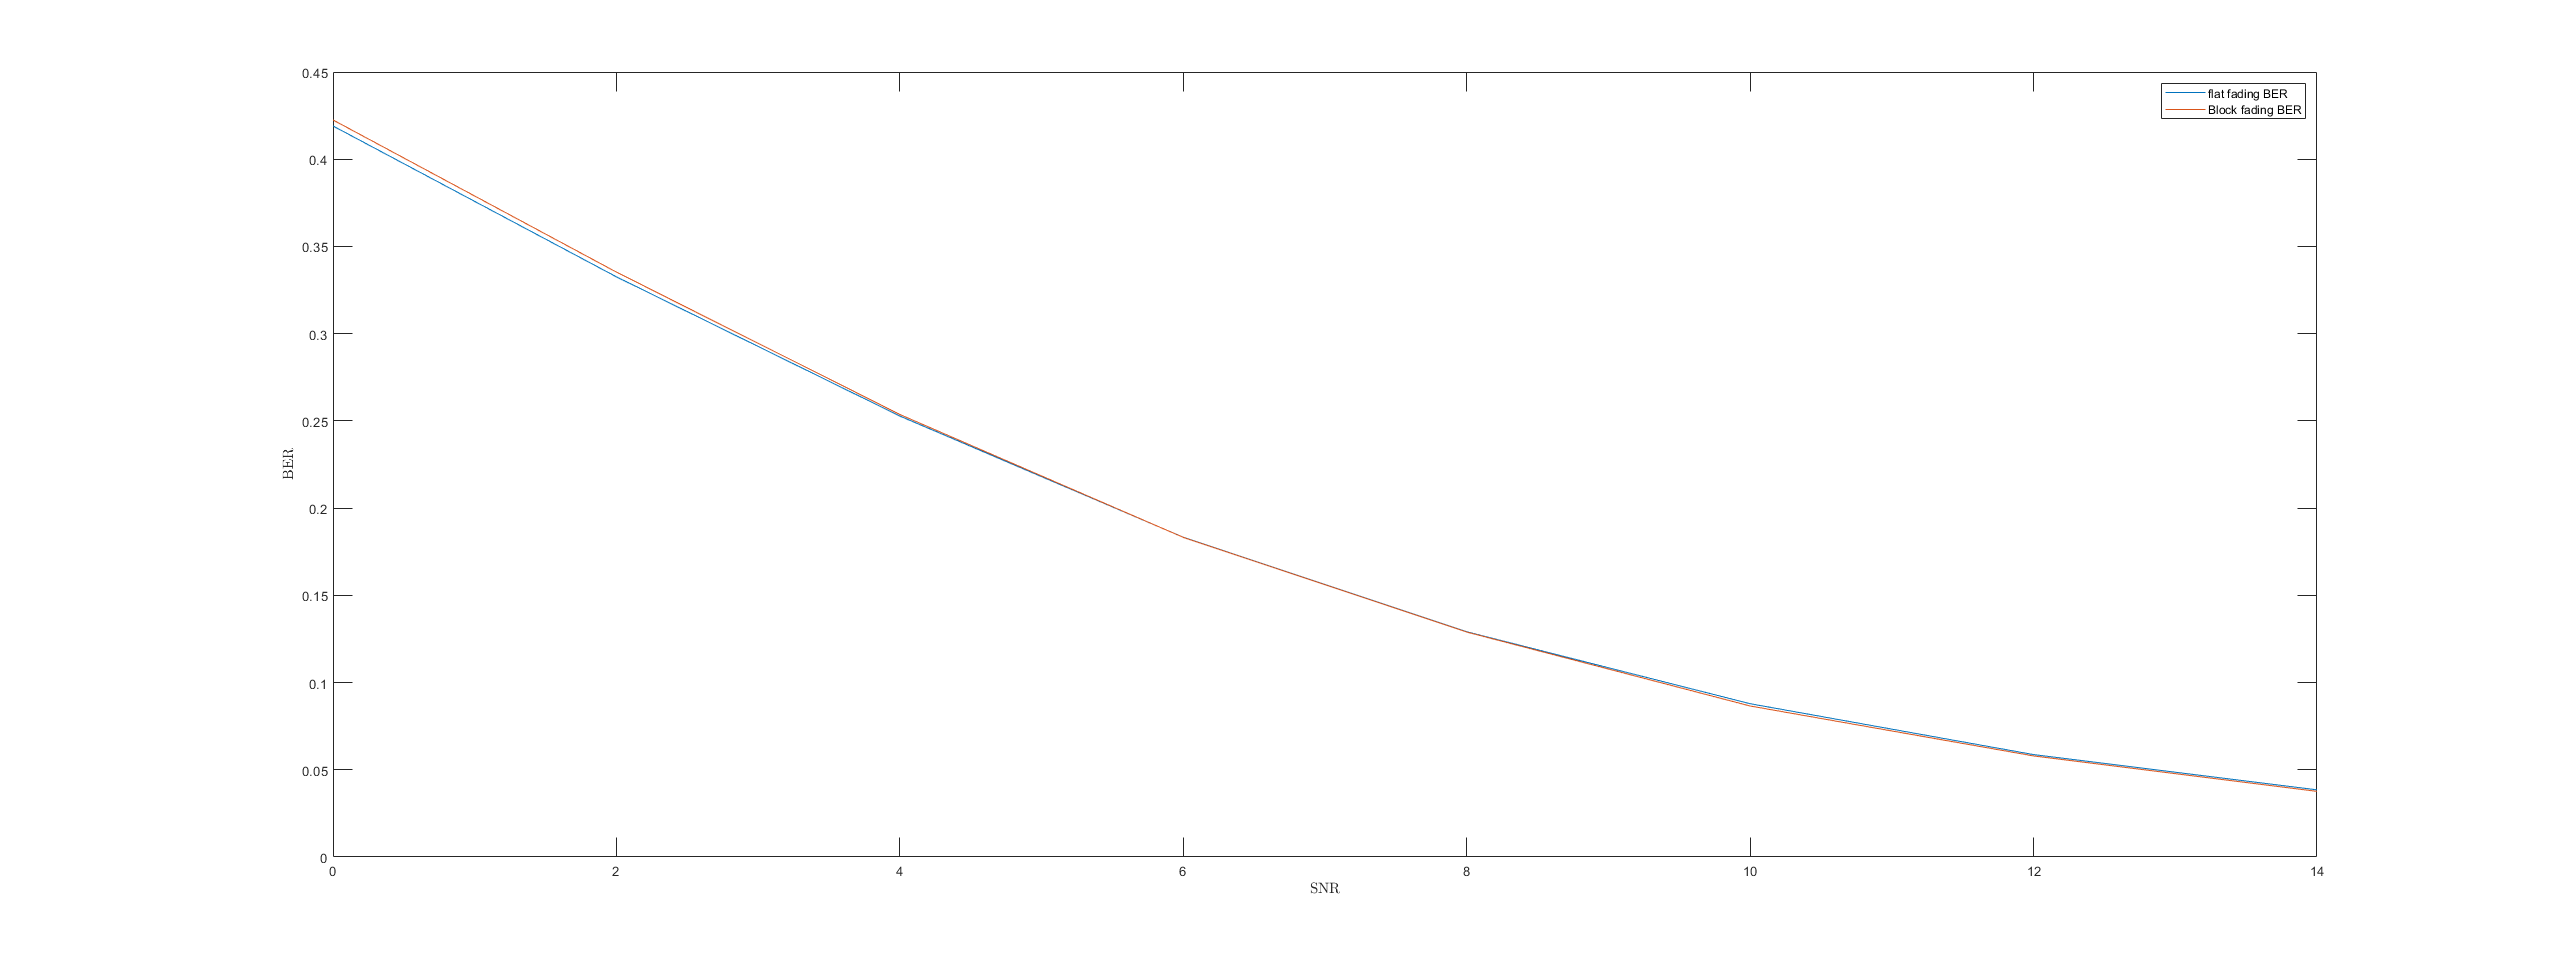
\includegraphics[width=0.9\textwidth]{fig6.png}
			\end{subfigure}
			\begin{subfigure}[b]{0.8\textwidth}
				\centering
				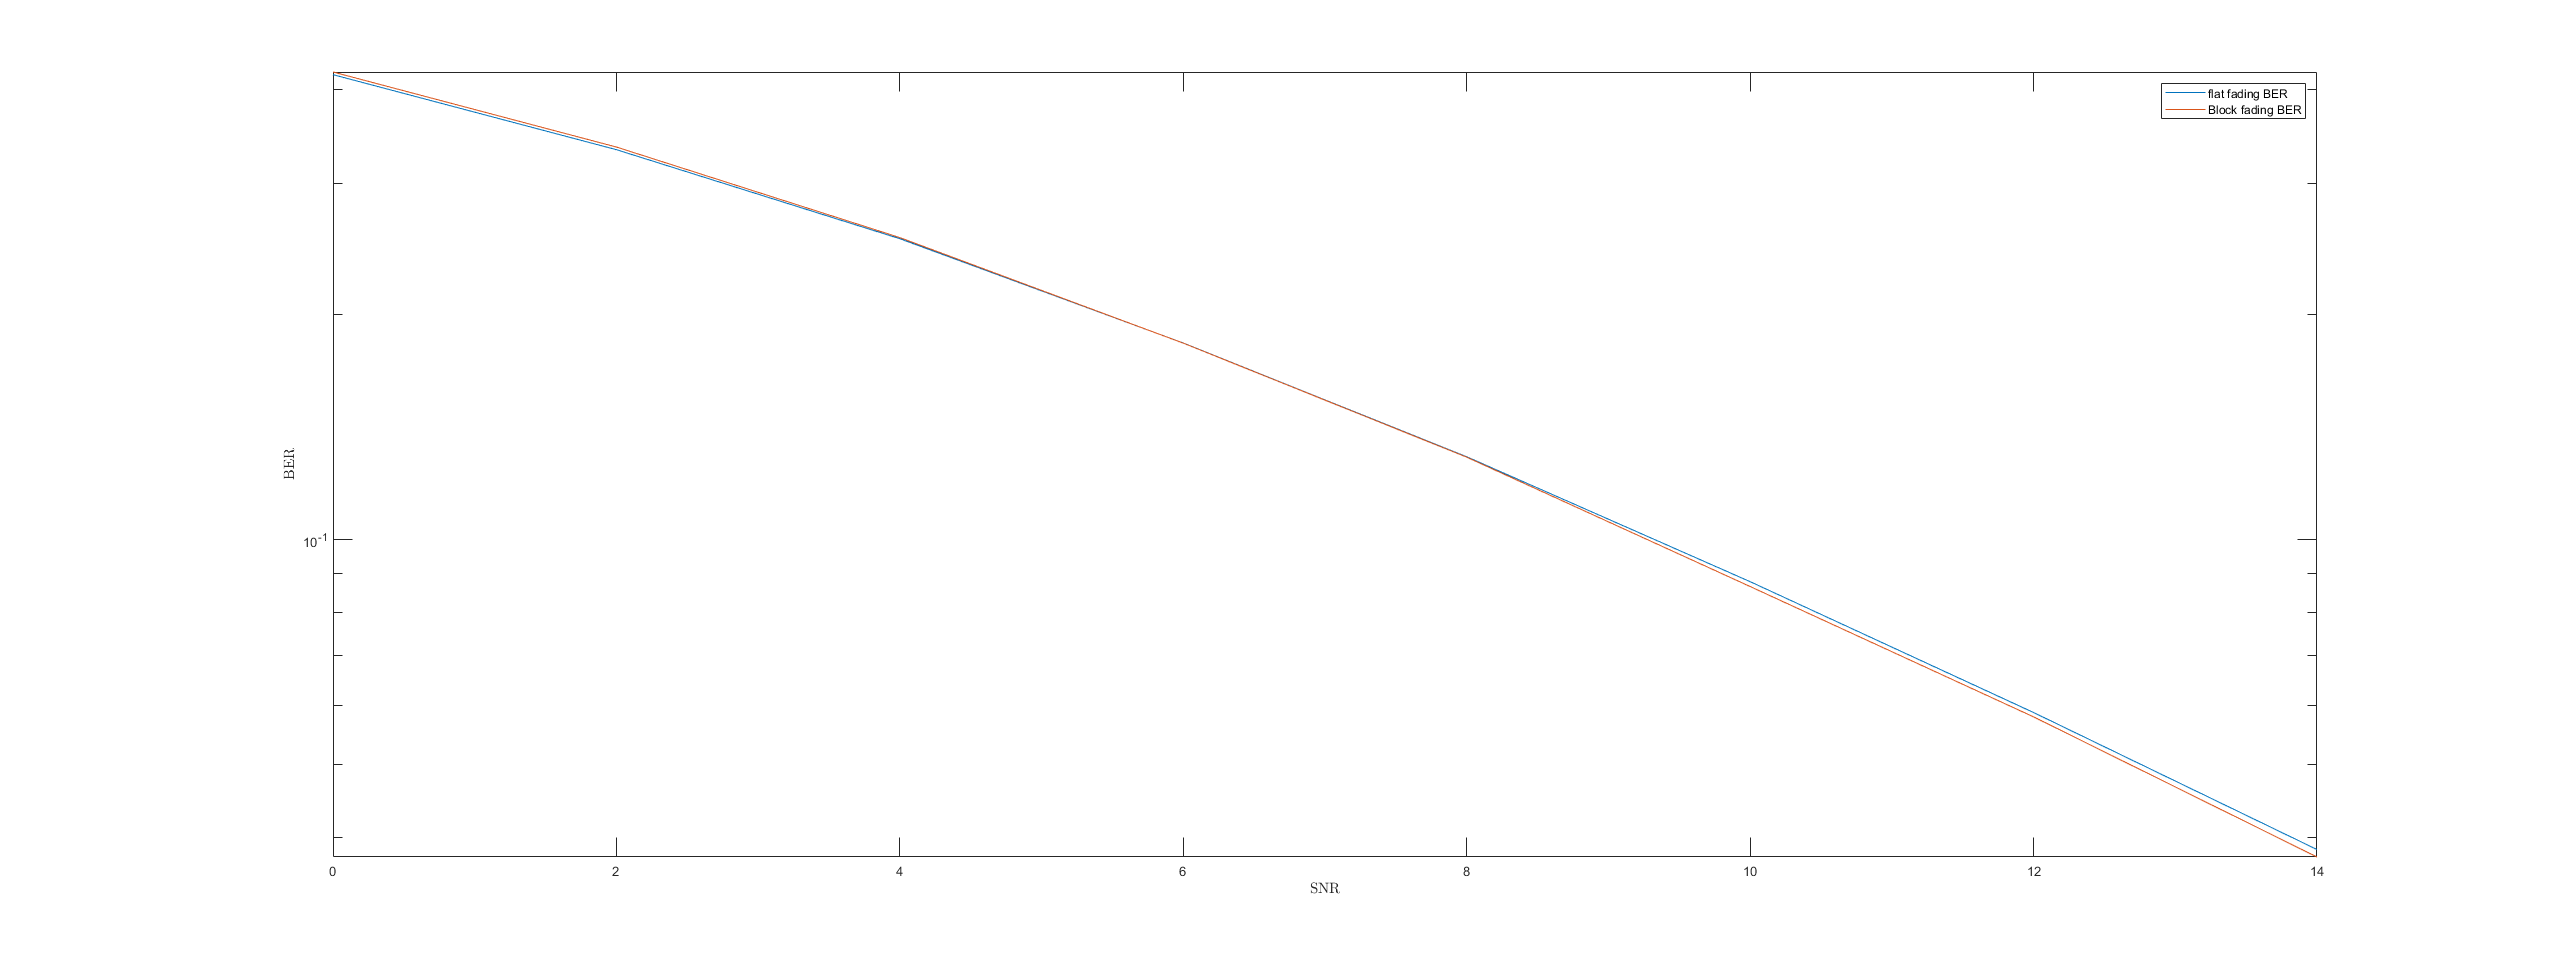
\includegraphics[width=0.9\textwidth]{fig7.png}
			\end{subfigure}
			\caption{$b\ll 1$}
		\end{figure}
	
		\begin{figure}[h!]
			\centering
			\begin{subfigure}[b]{0.8\textwidth}
				\centering
				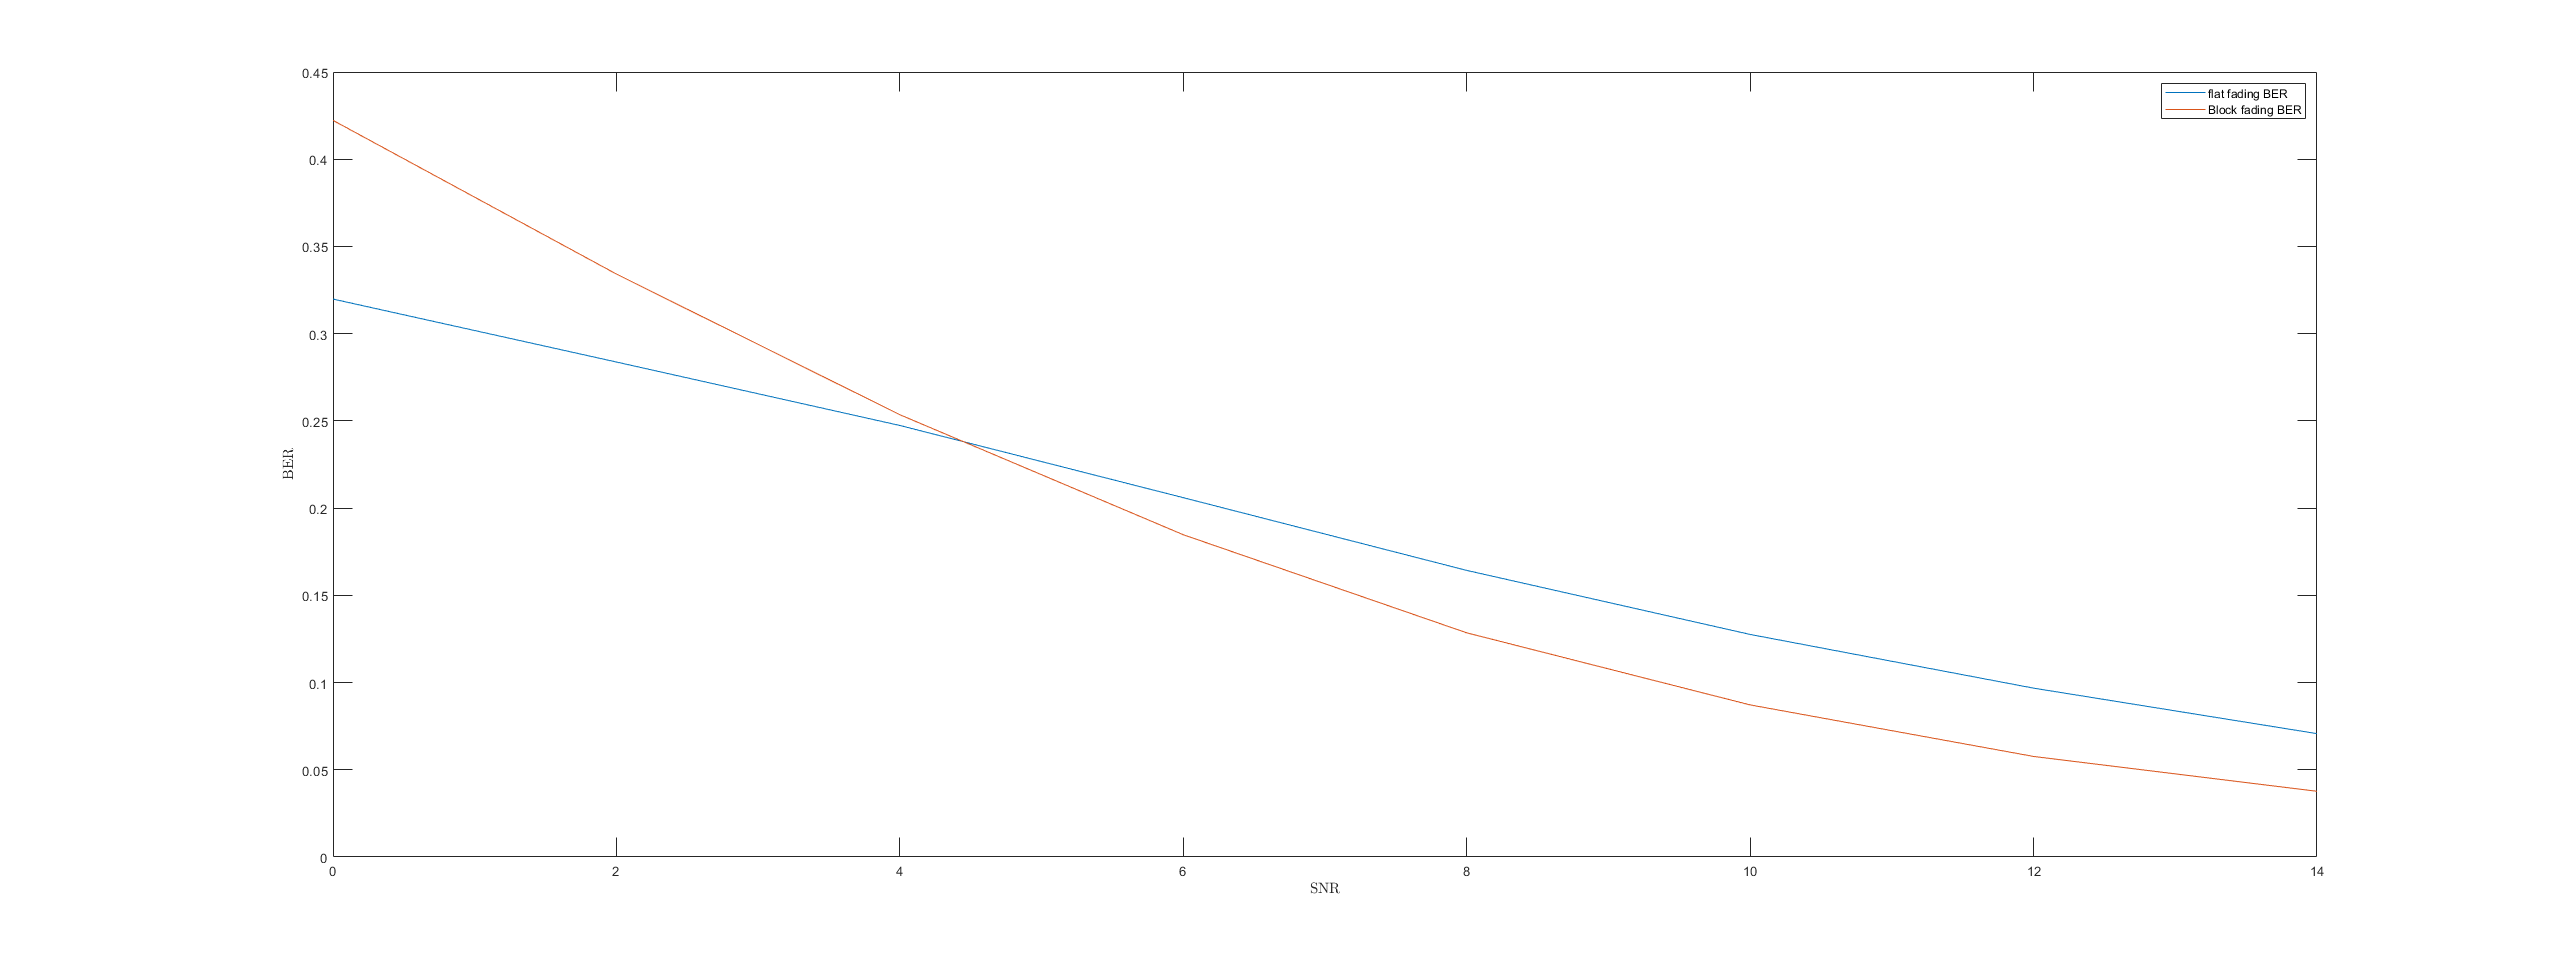
\includegraphics[width=0.9\textwidth]{fig6_b.png}
			\end{subfigure}
			\begin{subfigure}[b]{0.8\textwidth}
				\centering
				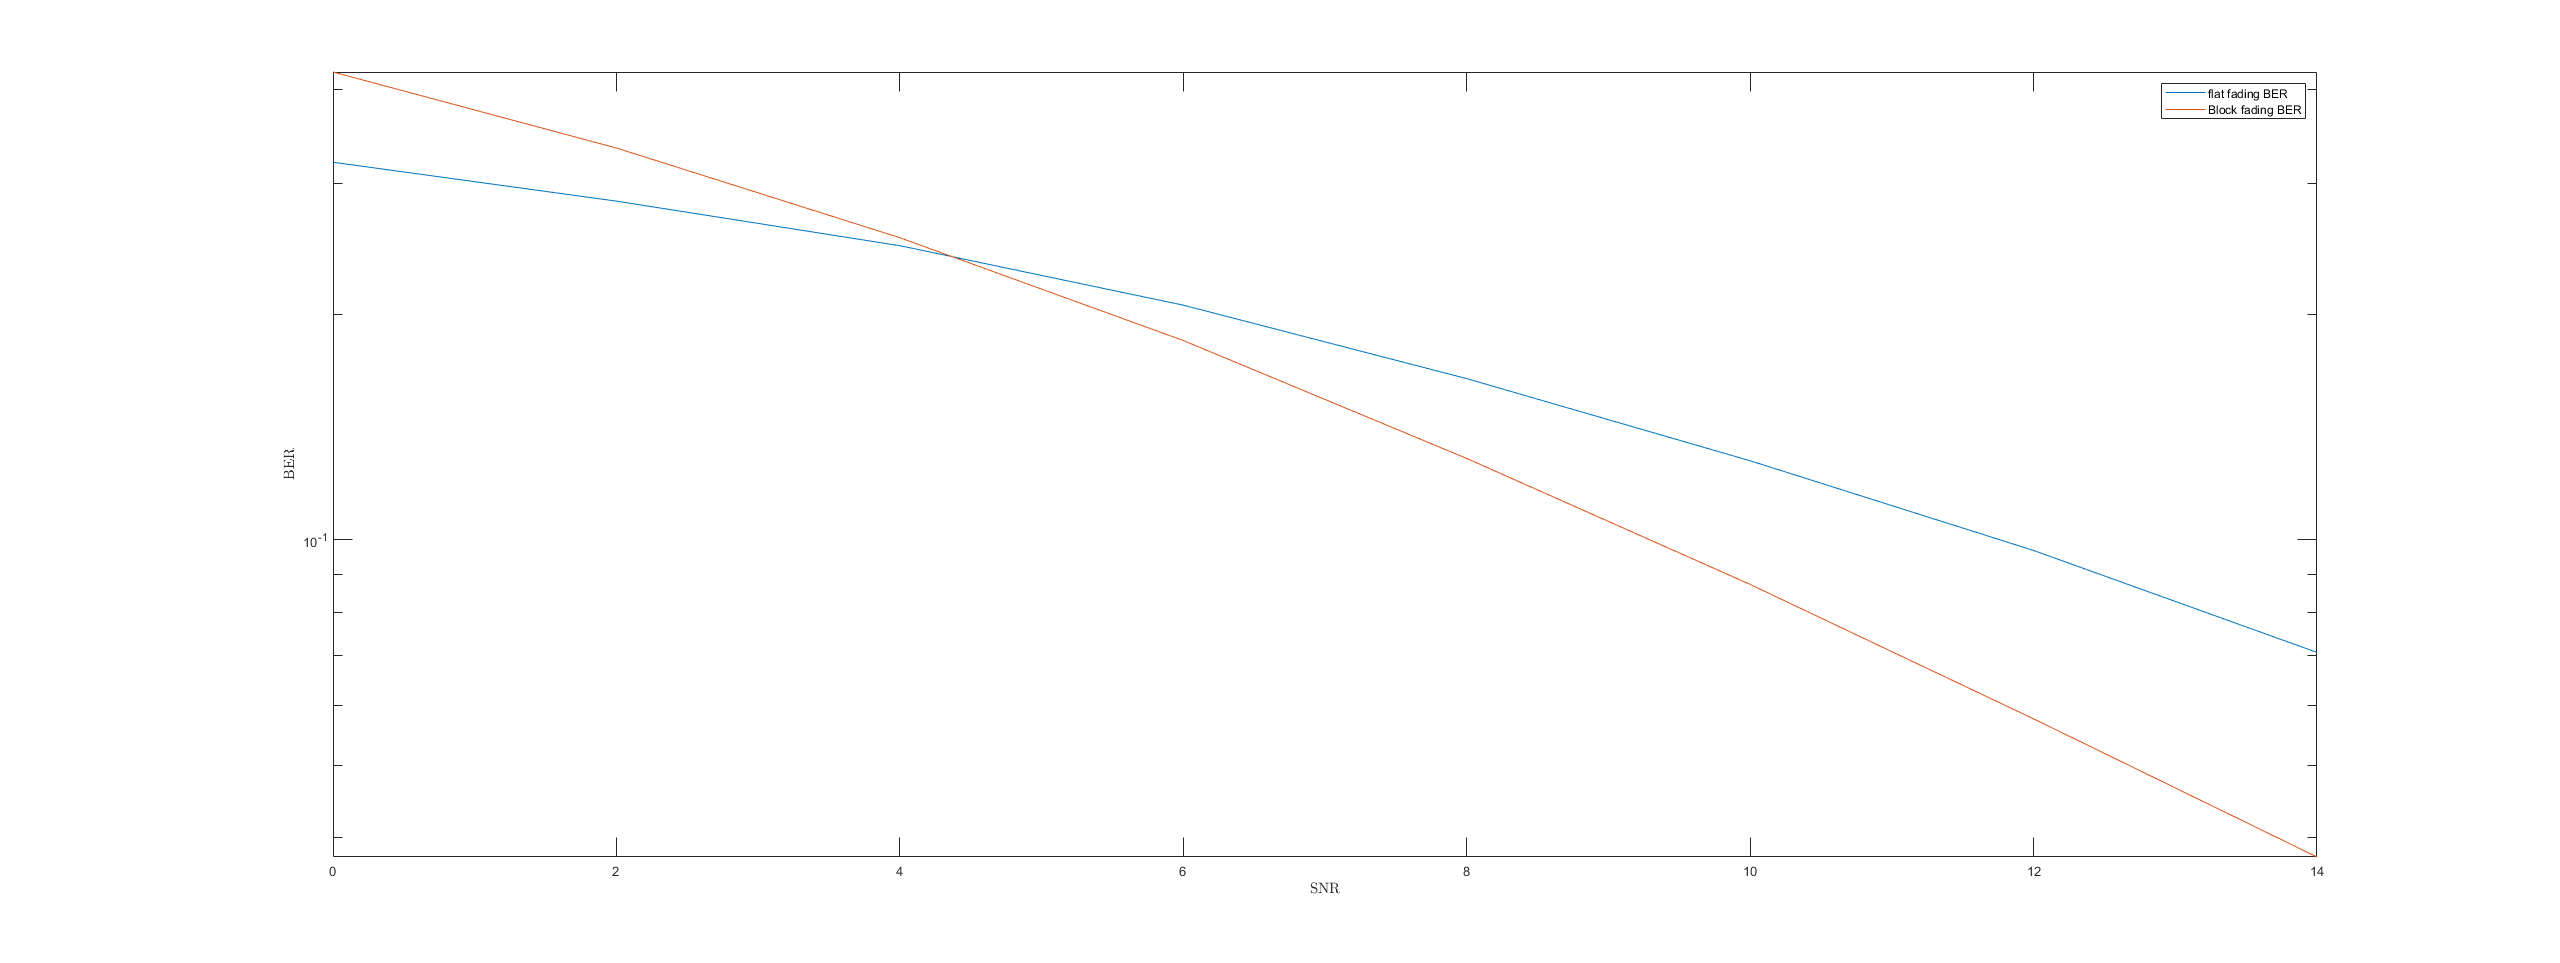
\includegraphics[width=0.9\textwidth]{fig7_b.png}
			\end{subfigure}
			\caption{$b\approx 1$ for first samples of $h$}
		\end{figure}
	
		\begin{figure}[h!]
			\centering
			\begin{subfigure}[b]{0.8\textwidth}
				\centering
				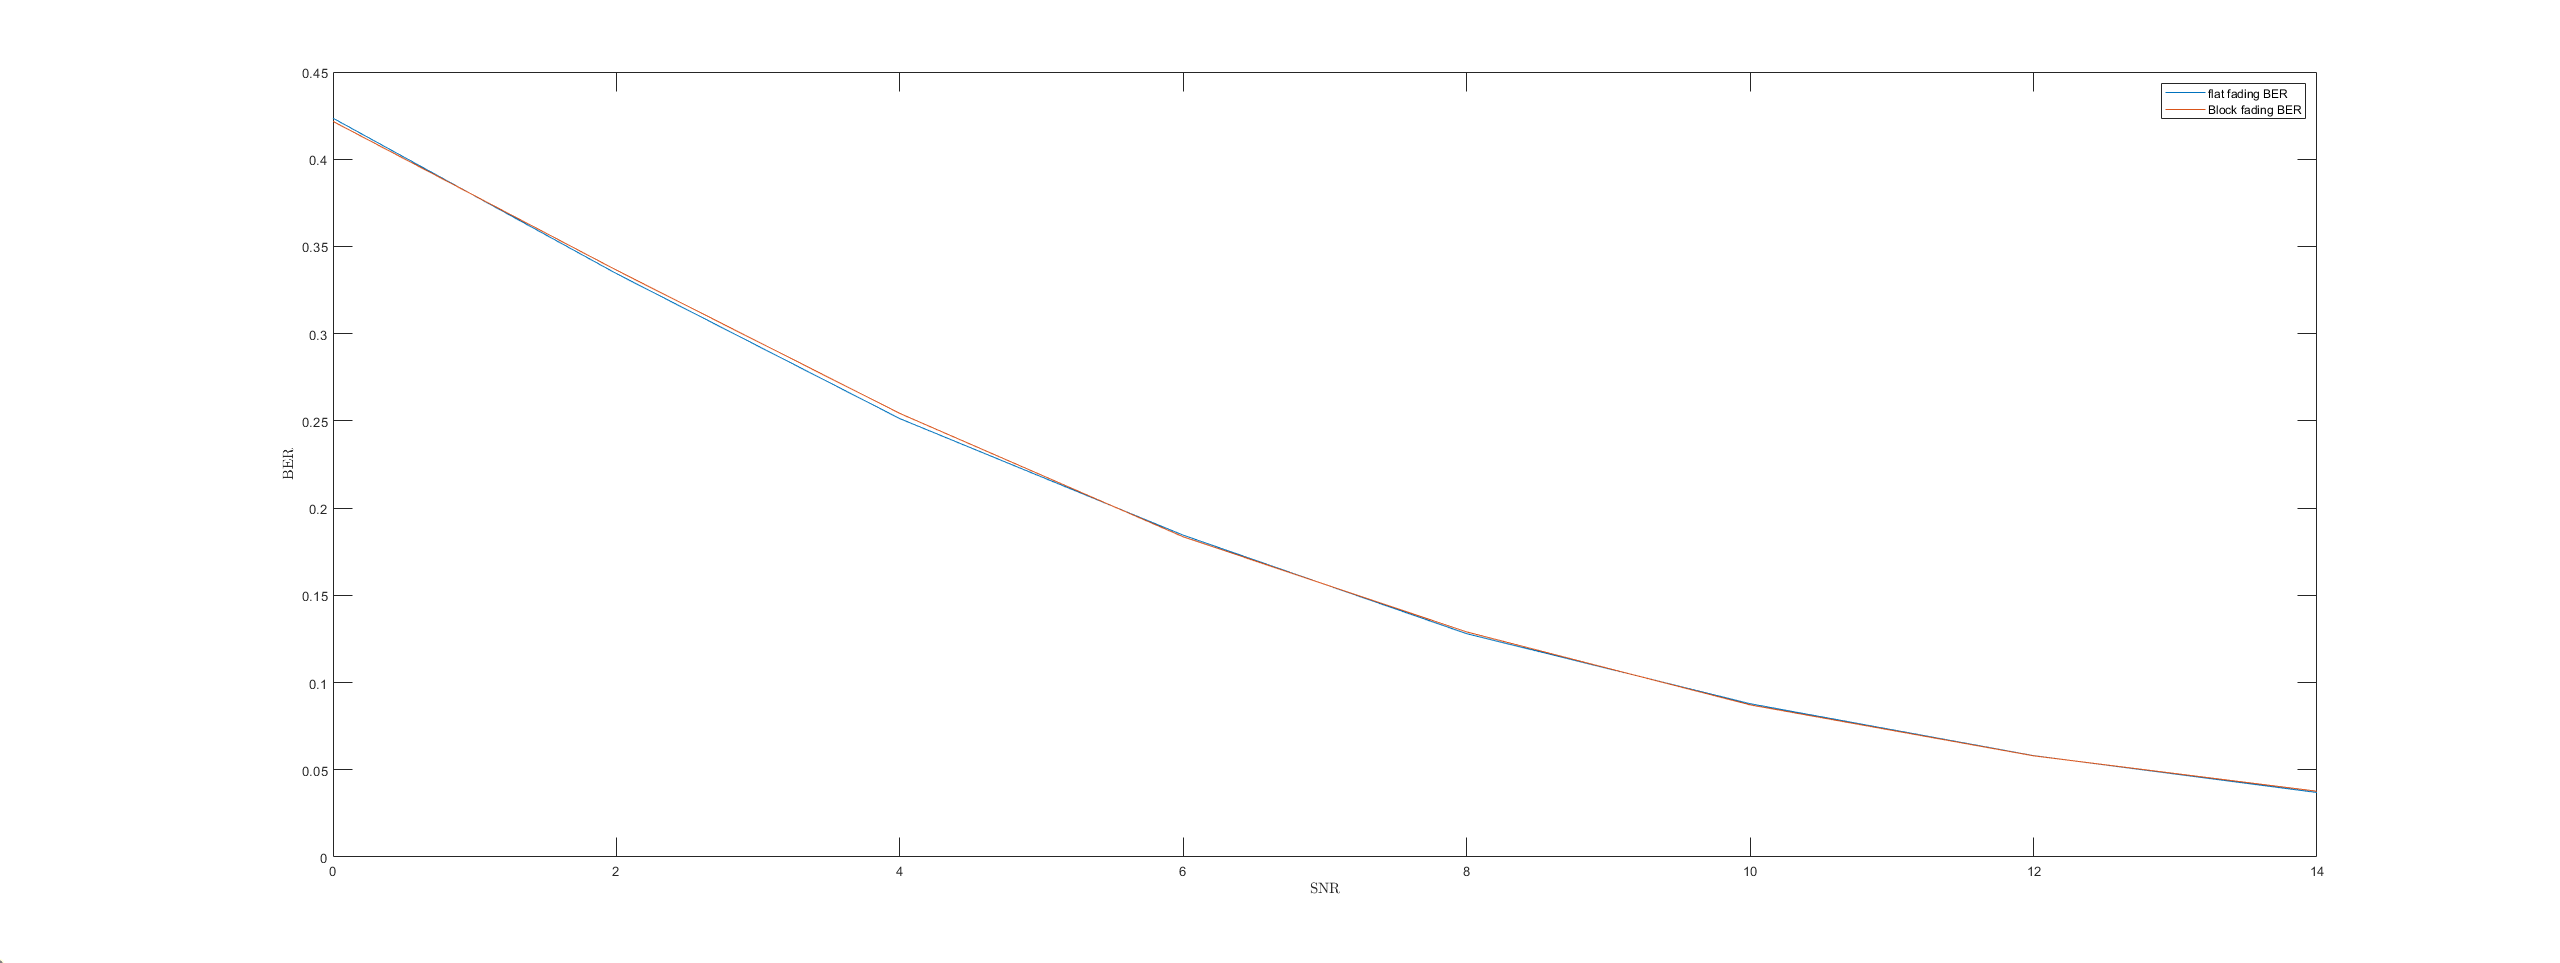
\includegraphics[width=0.9\textwidth]{fig8.png}
			\end{subfigure}
			\begin{subfigure}[b]{0.8\textwidth}
				\centering
				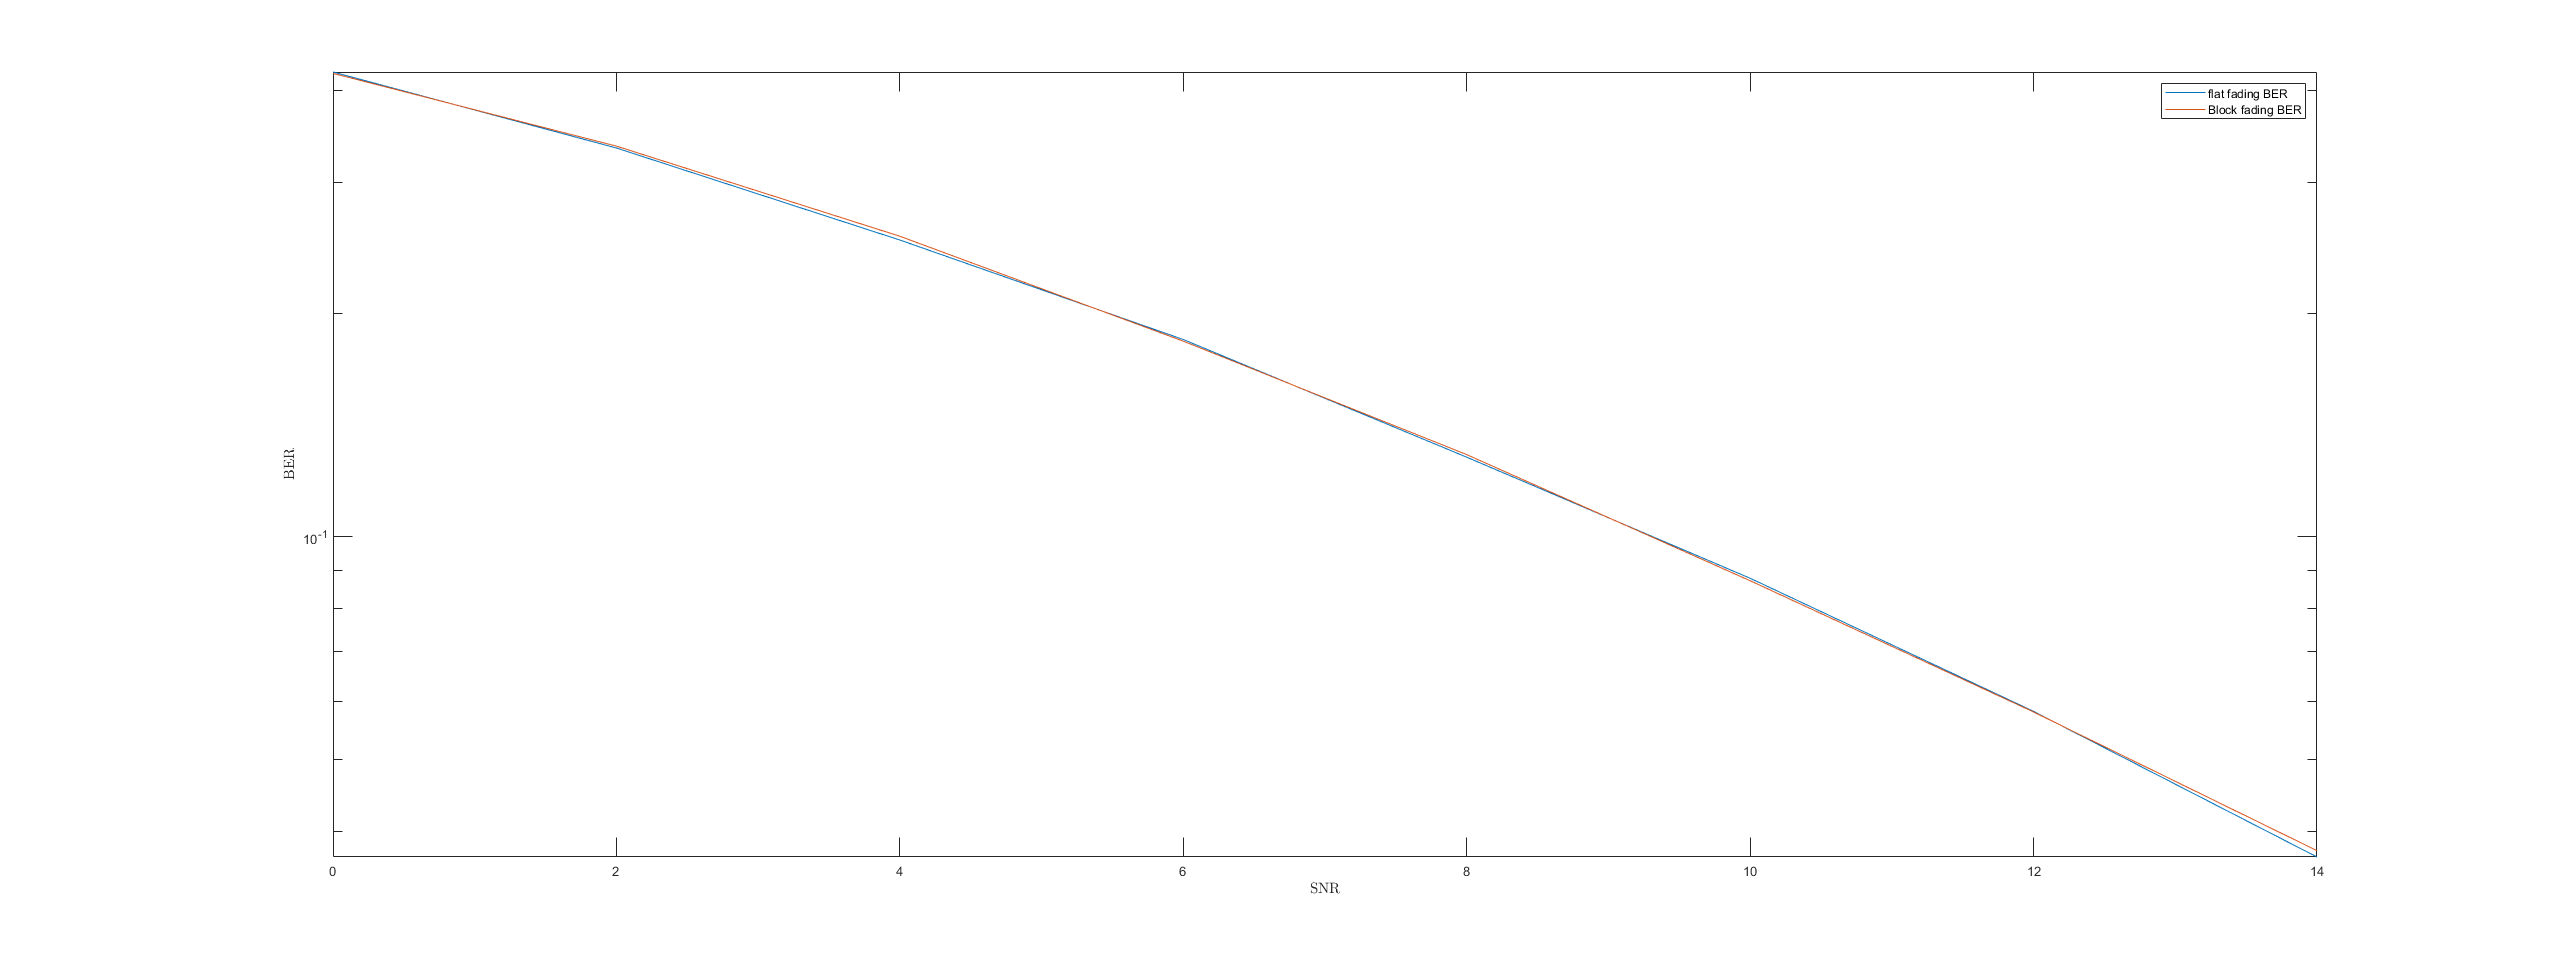
\includegraphics[width=0.9\textwidth]{fig8_b.png}
			\end{subfigure}
			\caption{$b\approx 1$ for later samples of $h$}
		\end{figure}
		\item[\bf 9]
		According to figure 6, we discern that when $b\ll1$ and therefore the flat fading channel is stationary, the two channels have comparable performance.\\
		By observing figures 7 and 8 for $b\approx$, if the flat fading channel hast become stationary yet the block fading one provides better performance for higher snrs. Although if the the channel has become stationary the performances are again comparable.
	\end{enumerate}
	
\end{document}
